%% Preamble 
\documentclass[11pt,a4paper]{article}
\usepackage[utf8]{inputenc}
\usepackage[T1]{fontenc}
\usepackage{lmodern}
\usepackage[margin=25mm]{geometry}
\usepackage{amsmath,amssymb,mathtools,bm,array,xcolor,booktabs,longtable}
\usepackage{tikz,microtype,enumitem}
\usepackage[nolist]{acronym}
\usetikzlibrary{arrows.meta,positioning,fit}
\usepackage[colorlinks=true,linkcolor=blue!50!black,urlcolor=blue!50!black]{hyperref}
\newenvironment{example}[1]{\par\medskip\noindent\textbf{Worked example: #1.}\ }{\par\medskip}
\setlist[itemize]{noitemsep}
\numberwithin{equation}{section}
\setcounter{tocdepth}{1}

%%%%%%%%%%%%%%%%%%%%%%%%%%%%%%%%%%%%%%%%%%%%%%%%%%%%%%%%%%%%
% MIMO Communications - Common LaTeX Commands
%%%%%%%%%%%%%%%%%%%%%%%%%%%%%%%%%%%%%%%%%%%%%%%%%%%%%%%%%%%%
% Required packages:
% \usepackage{amsmath,amssymb,amsfonts}
% \usepackage{mathtools}
% \usepackage{bm}
% \usepackage{array}
% \usepackage{xcolor}
%
% Convention:
% - Scalars: italic
% - Vectors/matrices: bold lowercase/uppercase
% - Sets: calligraphic
% - Descriptive indices: \mathsf
% - Matrix transpose markers: \mathsf
% - Named mathematical operators: upright
%%%%%%%%%%%%%%%%%%%%%%%%%%%%%%%%%%%%%%%%%%%%%%%%%%%%%%%%%%%%


%%%%%%%%%%%%%%%%%%%%%%%%%%%%%%%%%%%%%%%%%%%%%%%%%%%%%%%%%%%%
% 1. REVIEW AND EDITING
%%%%%%%%%%%%%%%%%%%%%%%%%%%%%%%%%%%%%%%%%%%%%%%%%%%%%%%%%%%%

% Display old text [blue] and proposed text [red]
\newcommand{\Review}[2]{%
	{\color{blue}[#1]}{\color{red}[#2]}}

% Display corrected versions
\newcommand{\Fixed}[2]{%
	{\color{orange}[#1]}{\color{green}[#2]}}

% Show only the accepted version (first argument)
\newcommand{\Done}[2]{#1}

% Comments and notes
\newcommand{\Response}[1]{{\color{magenta}[#1]}}
\newcommand{\Note}[1]{{\color{blue}[#1]}}


%%%%%%%%%%%%%%%%%%%%%%%%%%%%%%%%%%%%%%%%%%%%%%%%%%%%%%%%%%%%
% 2. GENERAL UTILITIES
%%%%%%%%%%%%%%%%%%%%%%%%%%%%%%%%%%%%%%%%%%%%%%%%%%%%%%%%%%%%

% Fixed-width table columns with proper line breaks
\newcolumntype{C}[1]{>{\centering\arraybackslash}p{#1}}
\newcolumntype{R}[1]{>{\raggedleft\arraybackslash}p{#1}}
\newcolumntype{L}[1]{>{\raggedright\arraybackslash}p{#1}}

% Display literal LaTeX text
\newcommand{\ttplain}[1]{\texttt{\detokenize{#1}}}

% Underbraces for expressions in matrices/arrays
\newcommand{\undermat}[2]{%
	\makebox[0pt][l]{$%
		\smash{%
			\underbrace{%
				\phantom{\begin{matrix}#2\end{matrix}}%
			}_{\text{$#1$}}%
		}$}#2}

\newcommand{\coolunder}[2]{%
	\mathrlap{%
		\smash{%
			\underbrace{%
				\phantom{\begin{matrix}#2\end{matrix}}%
			}_{\mbox{$#1$}}%
		}%
	}#2}


%%%%%%%%%%%%%%%%%%%%%%%%%%%%%%%%%%%%%%%%%%%%%%%%%%%%%%%%%%%%
% 3. CROSS-REFERENCING
%%%%%%%%%%%%%%%%%%%%%%%%%%%%%%%%%%%%%%%%%%%%%%%%%%%%%%%%%%%%

\newcommand{\figref}[1]{Figure.~\ref{#1}}
\newcommand{\secref}[1]{Section~\ref{#1}}
\newcommand{\chapref}[1]{Chapter~\ref{#1}}
\newcommand{\theref}[1]{Theorem~\ref{#1}}
\newcommand{\appref}[1]{Appendix~\ref{#1}}
\newcommand{\tabref}[1]{Table~\ref{#1}}

% Define if not already provided by another package
\providecommand{\algref}[1]{}
\renewcommand{\algref}[1]{Algorithm~\ref{#1}}
% Additional packages for notation tables
\usepackage{longtable}
\usepackage{array}
%% MATH NOTATION
%%%%%%%%%%%%%%%%%%%%%%%%%%%%%%%%%%%%%%%%%%%%%%%%%%%%%%%%%%%%
% 4. MATHEMATICAL OPERATORS AND DELIMITERS
%%%%%%%%%%%%%%%%%%%%%%%%%%%%%%%%%%%%%%%%%%%%%%%%%%%%%%%%%%%%

% Ceiling and floor (mathtools)
\DeclarePairedDelimiter{\ceil}{\lceil}{\rceil}
\DeclarePairedDelimiter{\floor}{\lfloor}{\rfloor}

% Optimization operators
\DeclareMathOperator*{\argmax}{arg\,max}
\DeclareMathOperator*{\argmin}{arg\,min}
\DeclareMathOperator*{\argfirst}{arg\,first}

% Angle/phase of complex quantity
% Overrides any existing \ang definition
\providecommand{\ang}[1]{}
\renewcommand{\ang}[1]{%
	\operatorname{angle}\left(#1\right)}

% Definition symbol
\newcommand{\define}{\triangleq}

% Delimiters (legacy commands)
\newcommand{\LeftP}{\left\lbrace}
\newcommand{\RightP}{\right\rbrace}
\newcommand{\LeftPD}{\left(}
\newcommand{\RightPD}{\right)}

% Additional delimiters
\newcommand{\Abs}[1]{\left|#1\right|}
\newcommand{\inner}[2]{%
	\left\langle #1,#2\right\rangle}


%%%%%%%%%%%%%%%%%%%%%%%%%%%%%%%%%%%%%%%%%%%%%%%%%%%%%%%%%%%%
% 5. SETS AND NUMBER FIELDS
%%%%%%%%%%%%%%%%%%%%%%%%%%%%%%%%%%%%%%%%%%%%%%%%%%%%%%%%%%%%

\newcommand{\compl}{\mathbb{C}}   % Complex field
\newcommand{\real}{\mathbb{R}}    % Real field
\newcommand{\intg}{\mathbb{Z}}    % Integers
\newcommand{\galois}{\mathbb{F}_2} % Binary finite field

% Calligraphic sets
\newcommand{\set}[1]{\mathcal{#1}}


%%%%%%%%%%%%%%%%%%%%%%%%%%%%%%%%%%%%%%%%%%%%%%%%%%%%%%%%%%%%
% 6. VECTORS AND MATRICES
%%%%%%%%%%%%%%%%%%%%%%%%%%%%%%%%%%%%%%%%%%%%%%%%%%%%%%%%%%%%

% Bold lowercase vectors and uppercase matrices
\newcommand{\ma}[1]{\bm{#1}}

% Element indexing
\newcommand{\IndexM}[3]{#1\left[#2,#3\right]}
\newcommand{\IndexV}[2]{#1\left[#2\right]}

% Norms
\newcommand{\Norm}[1]{\left\|#1\right\|}
\newcommand{\NormTwo}[1]{\left\|#1\right\|_2}
\newcommand{\frob}[1]{\left\|#1\right\|_{\mathsf{F}}}

% Matrix operations
\newcommand{\inv}[1]{{#1}^{-1}}
\newcommand{\pinv}[1]{{#1}^{+}}        % Pseudoinverse
\newcommand{\mT}[1]{{#1}^{\mathsf{T}}} % Transpose
\newcommand{\mH}[1]{{#1}^{\mathsf{H}}} % Hermitian transpose
\newcommand{\mC}[1]{{#1}^{*}}         % Complex conjugate

% Matrix properties and functions
\newcommand{\trace}[1]{%
	\operatorname{tr}\left(#1\right)}
\newcommand{\rank}[1]{%
	\operatorname{rank}\left(#1\right)}
\newcommand{\Cond}[1]{%
	\operatorname{cond}\left(#1\right)}
\newcommand{\Det}[1]{%
	\operatorname{det}\left(#1\right)}
\newcommand{\diag}[1]{%
	\operatorname{diag}\left(#1\right)}

% Alias for compatibility
\newcommand{\diagM}[1]{\diag{#1}}

% Vector subspaces
\newcommand{\Span}[1]{%
	\operatorname{span}\left(#1\right)}
\newcommand{\Null}[1]{%
	\operatorname{null}\left(#1\right)}
\newcommand{\Range}[1]{%
	\operatorname{range}\left(#1\right)}

% Vectorization and reshaping
\newcommand{\Vect}[1]{%
	\operatorname{vec}\left(#1\right)}
\newcommand{\unvec}[3]{%
	\operatorname{unvec}_{#2\times #3}\left(#1\right)}

% Matrix products
\newcommand{\elemProd}[2]{#1\odot #2}
\newcommand{\elemDiv}[2]{#1\oslash #2}
\newcommand{\kronProd}[2]{#1\otimes #2}


%%%%%%%%%%%%%%%%%%%%%%%%%%%%%%%%%%%%%%%%%%%%%%%%%%%%%%%%%%%%
% 7. PROBABILITY AND STATISTICS
%%%%%%%%%%%%%%%%%%%%%%%%%%%%%%%%%%%%%%%%%%%%%%%%%%%%%%%%%%%%

% Expectation and variance
\newcommand{\Ex}[1]{%
	\mathbb{E}\left[#1\right]}
\newcommand{\Var}[1]{%
	\operatorname{Var}\left[#1\right]}

% Covariance and correlation
\newcommand{\Cov}[2]{%
	\operatorname{Cov}\left(#1,#2\right)}
\newcommand{\Corr}[2]{%
	\operatorname{Corr}\left(#1,#2\right)}

% Probability of an event
\newcommand{\Prob}[1]{%
	\Pr\left(#1\right)}

% Mean-square error
\newcommand{\MSE}[1]{%
	\operatorname{MSE}\left(#1\right)}

% Distribution notation
\newcommand{\Normal}{\mathcal{N}}
\newcommand{\CNormal}{\mathcal{CN}}

% Complex signal operations
\newcommand{\RE}[1]{%
	\operatorname{Re}\left\{#1\right\}}
\newcommand{\IM}[1]{%
	\operatorname{Im}\left\{#1\right\}}


%%%%%%%%%%%%%%%%%%%%%%%%%%%%%%%%%%%%%%%%%%%%%%%%%%%%%%%%%%%%
% 8. SIGNAL PROCESSING OPERATIONS
%%%%%%%%%%%%%%%%%%%%%%%%%%%%%%%%%%%%%%%%%%%%%%%%%%%%%%%%%%%%

% Fourier transform
\newcommand{\FT}[1]{%
	\mathcal{F}\left\{#1\right\}}

% Circular convolution
\newcommand{\circConv}[2]{#1\circledast #2}

% Modulo reduction notation
\newcommand{\modulo}[2]{%
	\left\langle #1\right\rangle_{#2}}

% Sinc function
\newcommand{\Sinc}[1]{%
	\operatorname{sinc}\left(#1\right)}


%%%%%%%%%%%%%%%%%%%%%%%%%%%%%%%%%%%%%%%%%%%%%%%%%%%%%%%%%%%%
% 9. MIMO DIMENSIONS AND INDICES
%%%%%%%%%%%%%%%%%%%%%%%%%%%%%%%%%%%%%%%%%%%%%%%%%%%%%%%%%%%%

% Subscripts t/r: transmit/receive interfaces
% Superscripts rf/a: RF-chain/antenna-element interfaces
% No superscript: effective digital signal ports
% S: number of data streams
%
% Descriptive indices are upright (\mathsf).
% Running mathematical indices are italic..

% Digital signal ports
\newcommand{\NT}{N_{\mathsf{t}}}
\newcommand{\NR}{N_{\mathsf{r}}}
\newcommand{\nT}{n_{\mathsf{t}}}
\newcommand{\nR}{n_{\mathsf{r}}}

% Data streams
\newcommand{\NS}{S}
\newcommand{\nS}{s}

% RF chains
\newcommand{\NTrf}{N_{\mathsf{t}}^{\mathsf{rf}}}
\newcommand{\NRrf}{N_{\mathsf{r}}^{\mathsf{rf}}}
\newcommand{\nTrf}{n_{\mathsf{t}}^{\mathsf{rf}}}
\newcommand{\nRrf}{n_{\mathsf{r}}^{\mathsf{rf}}}

% Physical antenna elements
\newcommand{\NTa}{N_{\mathsf{t}}^{\mathsf{a}}}
\newcommand{\NRa}{N_{\mathsf{r}}^{\mathsf{a}}}
\newcommand{\nTa}{n_{\mathsf{t}}^{\mathsf{a}}}
\newcommand{\nRa}{n_{\mathsf{r}}^{\mathsf{a}}}


%%%%%%%%%%%%%%%%%%%%%%%%%%%%%%%%%%%%%%%%%%%%%%%%%%%%%%%%%%%%
% 10. MIMO PRECODING AND COMBINING MATRICES
%%%%%%%%%%%%%%%%%%%%%%%%%%%%%%%%%%%%%%%%%%%%%%%%%%%%%%%%%%%%

% Digital precoding and combining
\newcommand{\FD}{\ma{F}_{\mathsf{D}}}
\newcommand{\WD}{\ma{W}_{\mathsf{D}}}

% Analog precoding and combining
\newcommand{\FA}{\ma{F}_{\mathsf{A}}}
\newcommand{\WA}{\ma{W}_{\mathsf{A}}}


% MIMO channel representations

\newcommand{\Ha}{\ma{H}_{\mathsf{a}}}
% Antenna-level channel (physical antenna elements)

\newcommand{\Hrf}{\ma{H}_{\mathsf{rf}}}
% Effective channel after analog TX/RX processing


% H_a: Physical antenna-to-antenna channel
% H_rf: Effective channel between RF-chain interfaces
% H: Effective channel between digital signal ports
% H_s: Effective channel between data streams
%
% H_rf = W_A^H H_a F_A
% H    = W_D^H H_rf F_D
% H_s  = W^H H F


\newcommand{\Hs}{\ma{H}_{\mathsf{s}}}
% Effective stream-level channel after digital
% precoding and combining

% Diversity and multiplexing performance
\providecommand{\odiv}{o_{\mathsf{div}}}   % Diversity order
\providecommand{\gmux}{g_{\mathsf{mux}}}   % Multiplexing gain


%%%%%%%%%%%%%%%%%%%%%%%%%%%%%%%%%%%%%%%%%%%%%%%%%%%%%%%%%%%%
% 11. SIGNAL ENERGY AND NOISE
%%%%%%%%%%%%%%%%%%%%%%%%%%%%%%%%%%%%%%%%%%%%%%%%%%%%%%%%%%%%

\newcommand{\Es}{E_{\mathsf{s}}} % Energy per symbol
\newcommand{\Ed}{E_{\mathsf{d}}} % Total energy

\newcommand{\Eb}{E_{\mathsf{b}}} % Energy per bit

% Noise power spectral density parameter
\newcommand{\Nzero}{N_{0}}

\newcommand{\Ptx}{P_{\mathsf{t}}}
\newcommand{\Prx}{P_{\mathsf{r}}}


%%%%%%%%%%%%%%%%%%%%%%%%%%%%%%%%%%%%%%%%%%%%%%%%%%%%%%%%%%%%
% 12. COMMUNICATION METRICS AND ALGORITHMS
%%%%%%%%%%%%%%%%%%%%%%%%%%%%%%%%%%%%%%%%%%%%%%%%%%%%%%%%%%%%

\newcommand{\SNR}{\mathsf{SNR}}
\newcommand{\SINR}{\mathsf{SINR}}
\newcommand{\CSI}{\mathsf{CSI}}

% Combining and precoding
\newcommand{\MRT}{\mathsf{MRT}}
\newcommand{\MRC}{\mathsf{MRC}}
\newcommand{\ZF}{\mathsf{ZF}}
\newcommand{\LMMSE}{\mathsf{LMMSE}}

% Additional commonly used methods
\newcommand{\LS}{\mathsf{LS}}
\newcommand{\MMSE}{\mathsf{MMSE}}
\newcommand{\ML}{\mathsf{ML}}
\newcommand{\MAP}{\mathsf{MAP}}
\newcommand{\RZF}{\mathsf{RZF}}





%%%%%%%%%%%%%%%%%%%%%%%%%%%%%%%%%%%%%%%%%%%%%%%%%%%%%%%%%%%%
% End of common notation
%%%%%%%%%%%%%%%%%%%%%%%%%%%%%%%%%%%%%%%%%%%%%%%%%%%%%%%%%%%%

% Channel-rank abbreviation consistent with Lecture 01: $\RH=R_{\ma{H}}$.
\providecommand{\RH}{R_{\ma{H}}}
\title{MIMO Communications\\Lecture 02: Point-to-Point MIMO Fundamentals}
\author{Ahmad Nimr}
\date{Winter Semester 2026/27}


\begin{document}
% Register shared acronyms after the document begins.
\begin{acronym}
	\acro{p2p}[P2P]{point-to-point}
	\acro{mimo}[MIMO]{multiple-input multiple-output}
	\acro{siso}[SISO]{single-input single-output}
	\acro{simo}[SIMO]{single-input multiple-output}
	\acro{miso}[MISO]{multiple-input single-output}
	\acro{mrc}[MRC]{maximum ratio combining}
	\acro{mrt}[MRT]{maximum ratio transmission}
	\acro{zf}[ZF]{zero forcing}
	\acro{lmmse}[LMMSE]{linear minimum mean-square error}
	\acro{mmse}[MMSE]{minimum mean-square error}
	\acro{svd}[SVD]{singular value decomposition}
	\acro{evd}[EVD]{eigenvalue decomposition}
	\acro{snr}[SNR]{signal-to-noise ratio}
	\acro{sinr}[SINR]{signal-to-interference-plus-noise ratio}
	\acro{csi}[CSI]{channel state information}
	\acro{csir}[CSIR]{channel state information at the receiver}
	\acro{csit}[CSIT]{channel state information at the transmitter}
	\acro{rf}[RF]{radio frequency}
	\acro{qpsk}[QPSK]{quadrature phase-shift keying}
	\acro{awgn}[AWGN]{additive white Gaussian noise}
	\acro{psd}[PSD]{power spectral density}
	\acro{map}[MAP]{maximum a posteriori}
	\acro{mse}[MSE]{mean squared error}
	\acro{ls}[LS]{least squares}
	\acro{ml}[ML]{maximum likelihood }
	\acro{bpsk}[BPSK]{binary phase-shift keying}
	\acro{iid}[IID]{independent and identically distributed}
	\acro{los}[LOS]{line of sight}
	\acro{ostbc}[OSTBC]{orthogonal space-time block code}
	\acro{stbc}[STBC]{space-time block code}
	\acro{dmt}[DMT]{diversity--multiplexing tradeoff}
	\acro{pdf}[PDF]{probability density function}
	\acro{mumimo}[MU-MIMO]{multiuser multiple-input multiple-output}
	\acro{ul}[UL]{uplink}
	\acro{dl}[DL]{downlink}
	\acro{fdma}[FDMA]{frequency-division multiple access}
	\acro{tdma}[TDMA]{time-division multiple access}
	\acro{sdma}[SDMA]{space-division multiple access}
	\acro{bs}[BS]{base station}
	\acro{mac}[MAC]{multiple-access channel}
	\acro{bc}[BC]{broadcast channel}
	\acro{rzf}[RZF]{regularized zero forcing}
	\acro{sic}[SIC]{successive interference cancellation}
	\acro{dpc}[DPC]{dirty-paper coding}
	\acro{dof}[DoF]{degrees of freedom}
	\acro{tdd}[TDD]{time-division duplex}
	\acro{fdd}[FDD]{frequency-division duplex}
	\acro{ap}[AP]{access point}
	\acro{cpu}[CPU]{central processing unit}
	\acro{comp}[CoMP]{coordinated multipoint}
	\acro{cscg}[CSCG]{circularly symmetric complex Gaussian}
	\acro{mu}[MU]{multi-user}
	\acro{se}[SE]{spectral efficiency}
\end{acronym}


\maketitle
\begin{abstract}
This lecture develops the signal processing and information-theoretic foundations of narrowband point-to-point \ac{mimo}. Starting from the digital model established in Lecture~01, this lecture derives \ac{mrc} and \ac{mrt}, examines \ac{zf} and \ac{lmmse} equalization, introduces \ac{stbc} through the Alamouti scheme, and uses the \ac{svd} to construct parallel spatial channels. Gaussian mutual information then connects channel rank, eigenmode power allocation, and capacity. Worked examples show when to concentrate power into one mode and when to transmit several streams. The channel is treated as fixed; statistical channel models and fading performance follow in Lecture~03.
\end{abstract}
\acresetall
\tableofcontents
\newpage

\section{Introduction and motivation}
\subsection{Learning objectives and prerequisites}
After this lecture, students should be able to formulate a dimensionally consistent \ac{p2p} \ac{mimo} transceiver; derive and normalize \ac{mrc} and \ac{mrt} weights; explain interference suppression and noise enhancement in \ac{zf} and \ac{lmmse}; encode and decode a two-antenna Alamouti block and identify its CSI and rate requirements; construct \ac{svd} eigenmodes; compute Gaussian achievable rates; and solve a small water-filling problem. We use the complex-vector, covariance, pseudoinverse, and \ac{svd} tools from Lecture~01. Detailed optimization arguments and tutorial answers support independent study.


\subsection{From digital ports to spatial streams}

A \ac{p2p} \ac{mimo} link connects one transmitter and one receiver, each having one or more digital signal ports. As introduced in Lecture~01, the numbers of transmit and receive ports are denoted by $\NT$ and $\NR$, respectively. These ports represent the interfaces of the effective digital channel and do not necessarily correspond one-to-one to physical antenna elements. All transmitted signals belong to the same link, and the received observations can be processed jointly. This distinguishes \ac{p2p} \ac{mimo} from the multiuser systems introduced later.

\begin{center}
	\begin{tabular}{llll}
		\toprule
		Configuration & Transmit ports & Receive ports & Maximum rank\\
		\midrule
		\acs{siso} & $\NT=1$ & $\NR=1$ & $1$\\
		\acs{simo} & $\NT=1$ & $\NR>1$ & $1$\\
		\acs{miso} & $\NT>1$ & $\NR=1$ & $1$\\
		\acs{mimo} & $\NT>1$ & $\NR>1$ & $\min(\NT,\NR)$\\
		\bottomrule
	\end{tabular}
\end{center}

The effective channel $\ma{H}\in\compl^{\NR\times\NT}$ has rank
\begin{equation}
	\RH=\rank{\ma{H}}\leq\min(\NT,\NR).
\end{equation}
This rank determines the number of independent spatial channel dimensions. In particular, \ac{simo} and \ac{miso} provide only one spatial dimension, although additional ports can improve communication performance.

The number of transmitted data streams is denoted by $\NS$. For independent linear stream recovery, the necessary condition is
\begin{equation}
	\boxed{\NS\leq\RH\leq\min(\NT,\NR).}
\end{equation}
However, the number of useful streams may be smaller than the channel rank, depending on the channel gains, available transmit energy, and receiver processing.

\paragraph{Three fundamental MIMO benefits.}
As discussed in Lecture~01, multiple spatial ports can be exploited for three different purposes:
\begin{itemize}
	\item \textbf{Array gain:} improving the received \ac{snr} through coherent transmission and/or combining.
	\item \textbf{Diversity gain:} improving reliability by exploiting different fading characteristics across spatial and/or temporal observations.
	\item \textbf{Spatial multiplexing:} transmitting multiple independent data streams over the same time-frequency resource.
\end{itemize}
These benefits are distinct but may coexist. This lecture  examines the corresponding signal processing techniques for a fixed channel realization, including transmit diversity through space-time coding. Their statistical performance under fading is investigated in Lecture~03.

\begin{example}{two ports do not guarantee two independent streams}
	Consider two channels with the same digital port configuration, $\NT=\NR=2$:
	\begin{equation}
		\ma{H}_1=\ma{I}_2,\qquad
		\ma{H}_2=\ma{1}_2\mT{\ma{1}_2}.
	\end{equation}
	The first channel has rank two and preserves two independent input dimensions. The second has rank one, since both receive ports observe the same linear combination of the transmitted signals. Thus, additional observations may improve the received \ac{snr}, but cannot recover the missing spatial dimension.
	
	The channels have different Frobenius norms. Therefore, a fair comparison of their achievable rates must also account for their channel gains. Section~\ref{sec:specialchannels} revisits this example under equal total channel gain.
\end{example}

\section{P2P MIMO system model}\label{sec:model}

\subsection{Channel hierarchy}
The course model distinguishes physical propagation, frontend processing, and stream processing, as illustrated in \figref{fig:channel_hierarchy}.
\begin{figure}[ht]
	\centering
	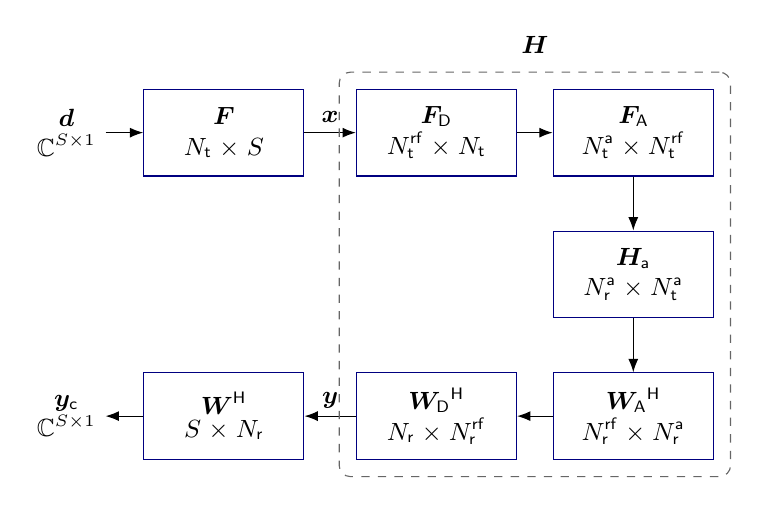
\begin{tikzpicture}[
		>=Latex,
		every node/.style={font=\small},
		blk/.style={draw=blue!50!black,align=center,minimum height=11mm,text width=18mm},
		sig/.style={align=center}
		]
		
		%------------------------------------------------
		% Stream processing (outside dashed box)
		%------------------------------------------------
		\node[sig] (d) at (-7.2,  1.8) {$\ma{d}$\\[0mm]$\compl^{\NS\times1}$};
		\node[blk] (F) at (-5.2,  1.8) {$\ma{F}$\\[0mm]$\NT\times\NS$};
		
		\node[blk] (W)  at (-5.2, -1.8) {$\mH{\ma{W}}$\\[-1mm]$\NS\times\NR$};
		\node[sig] (yc) at (-7.2, -1.8) {$\ma{y}_{\mathsf c}$\\[0mm]$\compl^{\NS\times1}$};
		
		%------------------------------------------------
		% Effective digital channel H (inside dashed box)
		%------------------------------------------------
		\node[blk] (FD) at (-2.5,  1.8) {$\FD$\\[0mm]$\NTrf\times\NT$};
		\node[blk] (FA) at ( 0.0,  1.8) {$\FA$\\[0mm]$\NTa\times\NTrf$};
		
		\node[blk] (Ha) at ( 0.0,  0.0) {$\Ha$\\[0mm]$\NRa\times\NTa$};
		
		\node[blk] (WA) at ( 0.0, -1.8) {$\mH{\WA}$\\[0mm]$\NRrf\times\NRa$};
		\node[blk] (WD) at (-2.5, -1.8) {$\mH{\WD}$\\[0mm]$\NR\times\NRrf$};
		
		% signal labels at interfaces
		\node[sig] (x) at (-3.85, 2) {$\ma{x}$};
		\node[sig] (y) at (-3.85,-1.6) {$\ma{y}$};
		
		%------------------------------------------------
		% Arrows
		%------------------------------------------------
		\draw[->] (d)  -- (F);
		\draw[->] (F)  -- (FD);
		\draw[->] (FD) -- (FA);
		\draw[->] (FA) -- (Ha);
		\draw[->] (Ha) -- (WA);
		\draw[->] (WA) -- (WD);
		\draw[->] (WD) -- (W);
		\draw[->] (W)  -- (yc);
		
		%------------------------------------------------
		% Dashed box for H only
		%------------------------------------------------
		\node[
		draw=black!60,
		dashed,
		rounded corners,
		fit=(FD)(FA)(Ha)(WA)(WD),
		inner sep=6pt,
		label={[yshift=1mm]above:$\ma{H}$}
		] {};
		
	\end{tikzpicture}
	\caption{Signal flow and channel hierarchy. The dashed box represents the effective digital channel $\ma{H}$.}
	\label{fig:channel_hierarchy}
\end{figure}
\newline
The antenna-domain channel is $	\Ha \in \compl^{\NRa \times \NTa}$. 
After analog frontend processing,
\begin{equation}\label{eq:Hrf_def}
	\boxed{
		\Hrf = \mH{\WA}\Ha\FA},
\end{equation}
with $\FA \in \compl^{\NTa \times \NTrf},
\WA \in \compl^{\NRa \times \NRrf},
\Hrf \in \compl^{\NRrf \times \NTrf}$. After digital frontend processing,
\begin{equation}\label{eq:H_def}
	\boxed{
		\ma{H} = \mH{\WD}\Hrf\FD},
\end{equation}
with $\FD \in \compl^{\NTrf \times \NT},
\WD \in \compl^{\NRrf \times \NR},
\ma{H} \in \compl^{\NR \times \NT}$. 
After stream precoding and combining,
\begin{equation}\label{eq:Hs_def}
	\boxed{
		\Hs = \mH{\ma{W}}\ma{H}\ma{F}},
\end{equation}
with $\ma{F} \in \compl^{\NT \times \NS},
\qquad
\ma{W} \in \compl^{\NR \times \NS},
\qquad
\Hs \in \compl^{\NS \times \NS}$.
\begin{center}
	\fbox{
		\parbox{0.92\linewidth}{
			\textbf{Lecture focus.}
			Lecture~02 starts from the effective digital channel $\ma{H}$ in \eqref{eq:H_def}. The frontend matrices $\FA$, $\WA$, $\FD$, and $\WD$ are treated as part of channel formation. The design variables in this part are the stream precoder $\ma{F}$ and combiner $\ma{W}$.
	}}
\end{center}

\paragraph{Examples of architectures.}

\begin{center}
	\small
	\begin{tabular}{@{}p{0.28\linewidth}
			p{0.40\linewidth}
			p{0.26\linewidth}@{}}
		\toprule
		Architecture & Frontend configuration & Effective channel\\
		\midrule
		Fully digital
		& Identity analog and digital frontends,
		$\NTrf=\NTa=\NT$,
		$\NRrf=\NRa=\NR$
		& $\ma{H}=\Hrf=\Ha$\\[1mm]
		
		Hybrid without digital frontend shaping
		& $\FD=\ma{I}_{\NT}$,
		$\WD=\ma{I}_{\NR}$
		& $\ma{H}=\Hrf$\\[1mm]
		
		General frontend shaping
		& Arbitrary compatible frontend matrices
		& $\ma{H}=\mH{\WD}\Hrf\FD$\\
		\bottomrule
	\end{tabular}
\end{center}


\subsection{Digital P2P MIMO model, stream precoding, and combining}

For the effective digital channel $\ma{H}$, the narrowband
complex-baseband model is
\begin{equation}\label{eq:model}
	\boxed{\ma{y}=\ma{H}\ma{x}+\ma{v}},
	\qquad
	\ma{v}\sim\CNormal(\ma{0},\sigma_v^2\ma{I}_{\NR}),
\end{equation}
where $\ma{x}\in\compl^{\NT\times1}$ and
$\ma{y},\ma{v}\in\compl^{\NR\times1}$.
The effective noise is assumed independent of the transmitted
signal and spatially and temporally white, with covariance
$\sigma_v^2\ma{I}_{\NR}$. Receiver frontend processing may
produce colored noise; this effect is neglected here.
\paragraph*{Whitening:} a non-white noise with covariance $\ma{R}_v$, the corresponding transformed white model is obtained as 
\begin{equation}
	\begin{split}
		\bar{\ma{y}} &= \ma{R}_v^{-1/2} \ma{y} \\
		&= \ma{R}_v^{-1/2} \ma{H} \ma{x} + \ma{R}_v^{-1/2} \ma{v}\\
		&= \bar{\ma{H}} \ma{x} + \bar{\ma{v}}.
	\end{split}
\end{equation} 
The transmit covariance and energy constraint are
\begin{equation}\label{eq:budget}
	\boxed{
		\ma{R}_x=\Ex{\ma{x}\mH{\ma{x}}}\succeq\ma{0},
		\qquad
		\trace{\ma{R}_x}\leq\Ed}.
\end{equation}
Here $\Ed$ denotes the total transmit-energy budget per
complex digital channel use. For energy-normalized pulses
and a power-preserving frontend,
\begin{equation*}
	\Ptx=\frac{\trace{\ma{R}_x}}{T_{\mathsf s}}
	\leq\frac{\Ed}{T_{\mathsf s}}.
\end{equation*}
In general, physical transmit power also depends on
frontend processing and normalization.

The reference \ac{snr} is defined as
\begin{equation}\label{eq:rho}
	\boxed{\rho\define\frac{\Ed}{\sigma_v^2}}.
\end{equation}

Consider $\NS$ independent, zero-mean data streams
$\ma{d}\in\compl^{\NS\times1}$ with covariance
\begin{equation}\label{eq:data_cov}
	\boxed{
		\ma{R}_d
		=\Ex{\ma{d}\mH{\ma{d}}}
		=\Ed\ma{I}_{\NS}}.
\end{equation}
Stream precoding and combining are defined by
\begin{align}
	\ma{x}&=\ma{F}\ma{d},
	&\ma{F}&\in\compl^{\NT\times\NS},
	\label{eq:stream_precoder}\\
	\ma{y}_{\mathsf c}&=\mH{\ma{W}}\ma{y},
	&\ma{W}&\in\compl^{\NR\times\NS}.
	\label{eq:stream_combiner}
\end{align}

The resulting transmit covariance is
\begin{equation*}
	\ma{R}_x
	=\ma{F}\ma{R}_d\mH{\ma{F}}
	=\Ed\ma{F}\mH{\ma{F}}.
\end{equation*}
Thus, the energy constraint in \eqref{eq:budget} becomes
\begin{equation}\label{eq:F_constraint}
	\boxed{\frob{\ma{F}}^2\leq1}.
\end{equation}

After receive combining,
\begin{equation}\label{eq:effective_stream_model}
	\boxed{
		\ma{y}_{\mathsf c}
		=\Hs\ma{d}+\ma{v}_{\mathsf c}},
\end{equation}
where
\begin{align*}
	\Hs&=\mH{\ma{W}}\ma{H}\ma{F},\\
	\ma{v}_{\mathsf c}&=\mH{\ma{W}}\ma{v}.
\end{align*}
The post-combining noise covariance is
\begin{equation}\label{eq:post_noise_cov}
	\ma{R}_{v_{\mathsf c}}
	=\Ex{\ma{v}_{\mathsf c}\mH{\ma{v}_{\mathsf c}}}
	=\sigma_v^2\mH{\ma{W}}\ma{W}.
\end{equation}

The vector $\ma{y}_{\mathsf c}$ contains soft stream
observations. If $\Hs=\ma{I}_{\NS}$, these are unbiased
linear estimates of $\ma{d}$.
The processed noise retains its original white covariance
when $\mH{\ma{W}}\ma{W}=\ma{I}_{\NS}$.
\figref{fig:digital_stream_model} illustrates the
corresponding signal processing model.
\begin{figure}[ht]
	\centering
	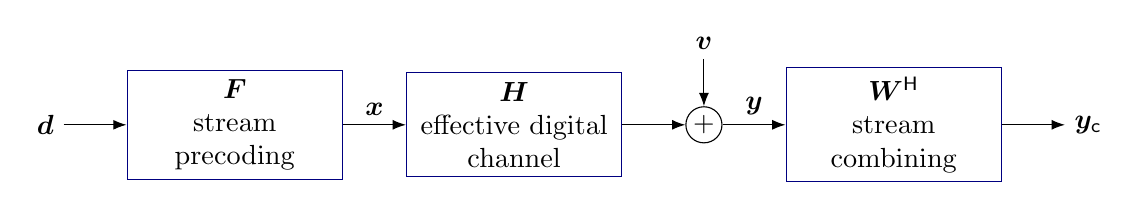
\begin{tikzpicture}[>=Latex,node distance=8mm,
		b/.style={draw=blue!50!black,align=center,minimum height=11mm,text width=25mm}]
		\node (d) {$\ma{d}$};
		\node[b,right=of d] (f) {$\ma{F}$\\stream\\precoding};
		\node[b,right=of f] (h) {$\ma{H}$\\effective digital\\channel};
		\node[right=of h,draw,circle,inner sep=1pt] (a) {$+$};
		\node[b,right=of a] (w) {$\mH{\ma{W}}$\\stream\\combining};
		\node[right=of w] (yc) {$\ma{y}_{\mathsf c}$};
		\node[above=6mm of a] (v) {$\ma{v}$};
		
		\draw[->] (d)--(f);
		\draw[->] (f)--node[above]{$\ma{x}$}(h);
		\draw[->] (h)--(a);
		\draw[->] (v)--(a);
		\draw[->] (a)--node[above]{$\ma{y}$}(w);
		\draw[->] (w)--(yc);
	\end{tikzpicture}
	\caption{Stream precoding and combining over the effective digital channel $\ma{H}$.}
	\label{fig:digital_stream_model}
\end{figure}

\begin{example}{dimensions and normalization}
	For $(\NT,\NR,\NS)=(4,3,2)$,
	\begin{equation*}
		\ma{F}\in\compl^{4\times2},\qquad
		\ma{W}\in\compl^{3\times2},\qquad
		\Hs\in\compl^{2\times2}.
	\end{equation*}
	Let $\ma{B}\in\compl^{4\times2}$ have orthonormal
	columns, $\mH{\ma{B}}\ma{B}=\ma{I}_2$.
	Equal-energy precoding gives
	\begin{equation*}
		\ma{F}=\frac{1}{\sqrt{2}}\ma{B},
		\qquad
		\frob{\ma{F}}^2=1,
		\qquad
		\trace{\ma{R}_x}=\Ed.
	\end{equation*}
	Without normalization, $\ma{F}=\ma{B}$ yields
	$\trace{\ma{R}_x}=2\Ed$, exceeding the budget.
\end{example}
\subsection{Channel state information}

\Ac{csir} denotes channel knowledge at the receiver, and \ac{csit} denotes channel knowledge at the transmitter.
\begin{itemize}
	\item \textbf{\acs{csir}:} required for coherent combining and equalization, including \ac{mrc}, \ac{zf}, and \ac{lmmse}.
	\item \textbf{\acs{csit}:} required for channel-adaptive precoding, including \ac{mrt}, \ac{svd} precoding, and water-filling.
\end{itemize}
Perfect \ac{csi} is assumed unless stated otherwise. Channel knowledge may be obtained through pilot-based estimation, feedback, or calibrated reciprocity. Without instantaneous \ac{csit}, the transmit covariance cannot depend on the channel realization.


\section{Linear transceiver processing}\label{sec:linear}

\subsection{SIMO: maximum-ratio combining}
For a single transmit port, let $x=d$, $\Ex{\Abs{d}^2}=\Ed$, and
$\ma{h}\in\compl^{\NR\times1}$. Linear combining gives
\begin{equation*}
	y_{\mathsf c}=\mH{\ma{w}}\ma{h}d+v_{\mathsf c},
	\qquad v_{\mathsf c}=\mH{\ma{w}}\ma{v},
\end{equation*}
with output \ac{snr}
\begin{equation}
	\SNR(\ma{w})
	=\frac{\Ed\Abs{\mH{\ma{w}}\ma{h}}^2}
	{\sigma_v^2\NormTwo{\ma{w}}^2} = \rho \frac{\Abs{\mH{\ma{w}}\ma{h}}^2}
	{\NormTwo{\ma{w}}^2}  .
\end{equation}
By Cauchy--Schwarz,
$\Abs{\mH{\ma{w}}\ma{h}}^2\leq
\NormTwo{\ma{w}}^2\NormTwo{\ma{h}}^2$,
with equality for $\ma{w}\propto\ma{h}$. Thus,
\begin{equation}\label{eq:mrc}
	\boxed{\ma{w}_{\MRC}=\frac{\ma{h}}{\NormTwo{\ma{h}}},
		\qquad \SNR_{\MRC}=\rho\NormTwo{\ma{h}}^2},
\end{equation}
where $\ma{h}\ne\ma{0}$. Unit-norm combining preserves noise
variance $\sigma_v^2$; alternative nonzero scalings leave the
\ac{snr} unchanged.

The corresponding Rayleigh quotient optimization
and the joint single-stream precoder/combiner
derivation are given in
Appendix~\ref{app:single-stream}.
\begin{example}{complex phases matter}
	For $\ma{h}=[1,j]^{\mathsf T}$,
	$\ma{w}_{\MRC}=[1,j]^{\mathsf T}/\sqrt{2}$ yields
	$y_{\mathsf c}=(y_1-jy_2)/\sqrt{2}=\sqrt{2}d+v_{\mathsf c}$
	and $\SNR_{\MRC}=2\rho$. By contrast,
	$\ma{w}=[1,1]^{\mathsf T}/\sqrt{2}$ yields $\SNR=\rho$.
\end{example}
For $\NR$ unit-magnitude channel coefficients, the received
\ac{snr} is $\NR\rho$. Its statistical diversity benefit is
addressed in Lecture~03.

\paragraph{Colored noise.}
For positive-definite $\ma{R}_v$,
\begin{equation}
	\SNR(\ma{w})
	=\frac{\Ed\Abs{\mH{\ma{w}}\ma{h}}^2}
	{\mH{\ma{w}}\ma{R}_v\ma{w}}  .
\end{equation}
the \ac{snr}-maximizing
combiner and its output \ac{snr} are
\begin{equation*}
	\ma{w}\propto\inv{\ma{R}_v}\ma{h},\qquad
	\SNR_{\max}=\Ed\mH{\ma{h}}\inv{\ma{R}_v}\ma{h}.
\end{equation*}

\subsection{MISO: maximum-ratio transmission}
For a single receive port, define $\ma{H}=\mT{\ma{h}}$,
where $\ma{h}\in\compl^{\NT\times1}$ contains the channel
coefficients. With $\ma{x}=\ma{f}d$ and $\NormTwo{\ma{f}}=1$,
\begin{equation*}
	y=\mT{\ma{h}}\ma{f}d+v,\qquad
	\SNR(\ma{f})=\rho\Abs{\mT{\ma{h}}\ma{f}}^2.
\end{equation*}
Cauchy--Schwarz gives
\begin{equation}\label{eq:mrt}
	\boxed{\ma{f}_{\MRT}=\frac{\mC{\ma{h}}}{\NormTwo{\ma{h}}},
		\qquad \SNR_{\MRT}=\rho\NormTwo{\ma{h}}^2}.
\end{equation}
\ac{mrt} requires instantaneous \ac{csit}. Unit-norm precoding
maintains the energy budget $\Ed$ independently of $\NT$.

\begin{example}{MRT and destructive transmission}
	For $\mT{\ma{h}}=[1,j]$, the choice
	$\ma{f}_{\MRT}=[1,-j]^{\mathsf T}/\sqrt{2}$ gives
	$\mT{\ma{h}}\ma{f}_{\MRT}=\sqrt{2}$ and $\SNR=2\rho$.
	Choosing $\ma{f}=[1,j]^{\mathsf T}/\sqrt{2}$ instead gives zero
	received signal gain.
\end{example}

\subsection{One stream over a general MIMO channel}
For unit-norm stream precoder $\ma{f}$ and combiner $\ma{w}$,
\begin{equation}\label{eq:single}
	\SNR=\rho\Abs{\mH{\ma{w}}\ma{H}\ma{f}}^2.
\end{equation}
For a fixed $\ma{f}$, \ac{mrc} gives
$\ma{w}\propto\ma{H}\ma{f}$. The remaining optimization is
\begin{equation*}
	\max_{\NormTwo{\ma{f}}=1}
	\mH{\ma{f}}\mH{\ma{H}}\ma{H}\ma{f}=\sigma_1^2.
\end{equation*}
Hence $\ma{f}=\ma{v}_1$ and $\ma{w}=\ma{u}_1$ yield
$\SNR_{\max}=\rho\sigma_1^2$, where $\sigma_1$ is the largest
singular value of $\ma{H}$. This maximizes single-stream \ac{snr},
not necessarily multistream sum rate.

\subsection{Multiple streams: interference and SINR}
Let $\ma{G}=\ma{H}\ma{F}=[\ma{g}_1,\ldots,\ma{g}_{\NS}]$,
with independent streams satisfying $\ma{R}_d=\Ed\ma{I}_{\NS}$.
The combined observation for stream $s$ is
\begin{equation*}
	y_{\mathsf c,s}
	=\mH{\ma{w}_s}\ma{g}_s d_s
	+\underbrace{\sum_{\ell\ne s}
		\mH{\ma{w}_s}\ma{g}_{\ell}d_{\ell}}_{z_s}
	+\mH{\ma{w}_s}\ma{v}.
\end{equation*}
The post-combining \ac{sinr} is
\begin{equation}\label{eq:sinr}
	\boxed{\rho_s = \SINR_s=
		\frac{\Ed\Abs{\mH{\ma{w}_s}\ma{g}_s}^2}
		{\Ed\sum_{\ell\ne s}
			\Abs{\mH{\ma{w}_s}\ma{g}_{\ell}}^2
			+\sigma_v^2\NormTwo{\ma{w}_s}^2}}.
\end{equation}
For independent proper Gaussian streams, separate decoding while
treating interstream interference as noise achieves
$\sum_{s=1}^{\NS}\log_2(1+\rho_s)$ bit per channel use.
This generally differs from the rate achievable with joint decoding.

\subsection{Zero-forcing equalization}
\ac{zf} enforces $\mH{\ma{W}_{\ZF}}\ma{G}=\ma{I}_{\NS}$,
requiring $\rank{\ma{G}}=\NS\leq\min(\NR,\RH)$.
The minimum-norm left inverse is
\begin{equation}\label{eq:zf}
	\boxed{\mH{\ma{W}_{\ZF}}=\pinv{\ma{G}}
		=\inv{(\mH{\ma{G}}\ma{G})}\mH{\ma{G}}}.
\end{equation}
The equalized observation and estimation-error covariance are
\begin{align*}
	\ma{y}_{\mathsf c}&=\ma{d}+\pinv{\ma{G}}\ma{v},\\
	\ma{R}_{\mathsf e,\ZF}
	&=\sigma_v^2\inv{(\mH{\ma{G}}\ma{G})}.
\end{align*}
Consequently,
\begin{equation}\label{eq:zfnoise}
	\boxed{\rho_{s,\ZF}=
		\frac{\Ed}{\sigma_v^2
			[\inv{(\mH{\ma{G}}\ma{G})}]_{ss}}}.
\end{equation}
Small singular values of $\ma{G}$ cause noise enhancement.
For rank-deficient $\ma{G}$, $\pinv{\ma{G}}\ma{G}$ is a
projection rather than the identity. Numerical implementations
prefer QR or \ac{svd} solutions over explicit matrix inversion.

\subsection{Linear minimum mean-square error equalization}
The \ac{lmmse} receiver minimizes
$\Ex{\NormTwo{\ma{d}-\ma{A}\ma{y}}^2}$ over
$\ma{A}=\mH{\ma{W}}$. With $\ma{R}_d=\Ed\ma{I}_{\NS}$,
the orthogonality principle yields
\begin{equation*}
	\Ex{(\ma{d}-\ma{A}\ma{y})\mH{\ma{y}}}=\ma{0},\qquad
	\ma{A}(\Ed\ma{G}\mH{\ma{G}}
	+\sigma_v^2\ma{I}_{\NR})=\Ed\mH{\ma{G}}.
\end{equation*}
Defining $\eta\define\sigma_v^2/\Ed = \frac{1}{\rho}$, the solution is
\begin{align}\label{eq:lmmse}
	\mH{\ma{W}_{\LMMSE}}
	&=\mH{\ma{G}}
	\inv{(\ma{G}\mH{\ma{G}}+\eta\ma{I}_{\NR})}\\
	&=\inv{(\mH{\ma{G}}\ma{G}+\eta\ma{I}_{\NS})}
	\mH{\ma{G}}.\nonumber
\end{align}
For arbitrary stream covariance and positive-definite noise
covariance, the general solution is
\begin{equation*}
	\mH{\ma{W}_{\LMMSE}}=\ma{R}_d\mH{\ma{G}}
	\inv{(\ma{G}\ma{R}_d\mH{\ma{G}}+\ma{R}_v)}.
\end{equation*}
\ac{lmmse} is optimal among linear estimators without requiring
Gaussian data. For jointly Gaussian streams and noise, it equals
the unrestricted \ac{mmse} estimator; minimum MSE does not in
general imply minimum symbol-error probability.

The estimation-error covariance is
\begin{equation}\label{eq:mmseerror}
	\boxed{\ma{R}_{\mathsf e,\LMMSE}
		=\Ed\inv{\left(\ma{I}_{\NS}
			+\rho\mH{\ma{G}}\ma{G}\right)}}.
\end{equation}
The effective gain $\ma{W}_{\LMMSE}\ma{G}$ is generally not
the identity, so estimation error includes gain shrinkage and
residual interference. For full-column-rank $\ma{G}$, the
\ac{lmmse} equalizer approaches \ac{zf} as $\eta\to0$; for
large $\eta$ it approaches a scaled matched filter.

\begin{example}{regularizing a weak stream}\label{ex:weak}
	Let $\ma{H}=\diag{1,0.1}$, $\Ed=1$,
	$\ma{F}=\ma{I}_2/\sqrt{2}$, and $\sigma_v^2=0.05$.
	Then $\frob{\ma{F}}^2=1$ and
	$\ma{G}=\diag{1,0.1}/\sqrt{2}$.
	The two equalizers are
	\begin{align*}
		\ma{W}_{\ZF}&=\sqrt{2}\diag{1,10},\\
		\ma{W}_{\LMMSE}&=\sqrt{2}\diag{10/11,10/11}.
	\end{align*}
	Their estimation-error covariances are
	\begin{align*}
		\ma{R}_{\mathsf e,\ZF}&=\diag{0.1,10},\\
		\ma{R}_{\mathsf e,\LMMSE}&=\diag{1/11,10/11}.
	\end{align*}
	The \ac{lmmse} effective gains are $10/11$ and $1/11$.
	Because the channel is diagonal, the two equalizers differ
	only by output scaling and yield the same stream SINRs:
	$10$ and $0.1$. Their MSEs differ substantially.
\end{example}

\paragraph{Design criteria and post-equalization SINR.}
\ac{zf} cancels interstream interference; \ac{lmmse} minimizes
sum estimation MSE. For independent Gaussian streams,
\begin{equation}\label{eq:mmse-sinr}
	\boxed{\rho_{s,\LMMSE}
		=\frac{\Ed}{[\ma{R}_{\mathsf e,\LMMSE}]_{ss}}-1}.
\end{equation}
The \ac{lmmse} output is a scaled maximum-\ac{sinr} linear
observation for each stream when the other streams are treated
as noise. Its output-noise variance alone does not determine
the \ac{sinr}, since residual interference may remain.
The \ac{lmmse} combiner also maximizes the
post-combining \ac{sinr} of each stream when
the remaining streams are treated as interference.
The corresponding derivation is given in
Appendix~\ref{app:sinr-lmmse}.
\section{Space-time block coding: transmit diversity}\label{sec:stbc}

\subsection{Motivation}
Linear precoding maps data streams into transmit signals within each channel use. \Ac{stbc} instead distributes information symbols across transmit ports and consecutive channel uses to improve reliability under fading. In contrast to spatial multiplexing, an \ac{stbc} does not necessarily increase the number of independent information symbols per channel use. Its main benefit appears under fading and is quantified in Lecture~03.

Consider a two-transmit-port, \(N_{\mathsf r}\)-receive-port link with effective digital  channel
\begin{equation*}
\ma{H} = \begin{bmatrix}\ma{h}_1 & \ma{h}_2\end{bmatrix}\in\compl^{\NR\times 2}, ~ \ma{h}_1, \ma{h}_2 \in \compl^{\NR \times 1}.
\end{equation*}
Assume a frequency-flat channel that remains constant over two consecutive channel uses, perfect \ac{csir}, no instantaneous \ac{csit}, and temporally white proper Gaussian noise with variance \(\sigma_v^2\) per use. The total transmit-energy budget is \(\Ed\) per channel use, summed over both antennas.

\subsection{Alamouti code for two transmit ports}
Let
\[
\ma{d}=\begin{bmatrix}d_1\\d_2\end{bmatrix},
\qquad
\Ex{\Abs{d_1}^2}=\Ex{\Abs{d_2}^2}=\Ed.
\]
The Alamouti codeword is
\begin{equation}\label{eq:alamouti-block}
	\boxed{
		\ma{X}
		=\frac{1}{\sqrt{2}}
		\begin{bmatrix}
			d_1 & d_2\\
			-d_2^* & d_1^*
	\end{bmatrix}},
\end{equation}
where rows correspond to consecutive channel uses and columns to transmit antennas.The factor \(1/\sqrt{2}\) ensures an average transmit energy of \(E_{\mathsf d}\) per channel use, equally distributed over both transmit ports. The code transmits two complex symbols in two channel uses, hence its code rate is
\[
R_{\mathsf{code}}=1
\quad \text{complex symbol per channel use.}
\]
The received samples are
\begin{align*}
	\ma{y}_1&=\frac{1}{\sqrt{2}}(\ma{h}_1d_1+\ma{h}_2d_2)+\ma{v}_1 \in \compl^{\NR\times 1},\\
	\ma{y}_2&=\frac{1}{\sqrt{2}}(-\ma{h}_1d_2^*+\ma{h}_2d_1^*)+\ma{v}_2 \in \compl^{\NR\times 1}.
\end{align*}
Stacking $\ma{y}_1$ and $\ma{y}_2^*$ gives the equivalent linear model
\begin{equation}\label{eq:alamouti-equiv}
	\boxed{
		\ma{y}_{\mathsf A}
		=\frac{1}{\sqrt{2}}\ma{H}_{\mathsf A}\ma{d}
		+\ma{v}_{\mathsf A}} \in \compl^{2\NR\times 1},
\end{equation}
with
\[
\ma{y}_{\mathsf A}\define
\begin{bmatrix}\ma{y}_1\\\ma{y}_2^*\end{bmatrix},
\qquad
\ma{v}_{\mathsf A}\define
\begin{bmatrix}\ma{v}_1\\\ma{v}_2^*\end{bmatrix},
\qquad
\ma{H}_{\mathsf A}\define
\begin{bmatrix}
\ma{h}_1 &\ma{h}_2\\
	\ma{h}_2^* & -\ma{h}_1^*
\end{bmatrix} \in \compl^{2\NR\times 2}.
\]
The equivalent channel has orthogonal columns:
\begin{equation}\label{eq:alamouti-orth}
	\boxed{
		\mH{\ma{H}_{\mathsf A}}\ma{H}_{\mathsf A}
		= \left(\NormTwo{\ma{h}_1}^2+\NormTwo{\ma{h}_2}^2\right)\ma{I}_2 = \frob{\ma{H}}^2\ma{I}_2.
	}
\end{equation}

\subsection{Linear combining, SNR, and rate}

Multiplying \eqref{eq:alamouti-equiv} by
$\mH{\ma{H}_{\mathsf A}}$ gives
\begin{equation*}
	\ma{y}_{\mathsf c}
	=\frac{\frob{\ma{H}}^2}{\sqrt{2}}\ma{d}
	+\ma{v}_{\mathsf c},
	\qquad
	\ma{v}_{\mathsf c}
	=\mH{\ma{H}_{\mathsf A}}\ma{v}_{\mathsf A}.
\end{equation*}
Since
\begin{equation*}
	\ma{R}_{v_{\mathsf A}}
	=\sigma_v^2\ma{I}_{2\NR},
\end{equation*}
the post-combining noise covariance is
\begin{equation*}
	\ma{R}_{v_{\mathsf c}}
	=\sigma_v^2
	\mH{\ma{H}_{\mathsf A}}\ma{H}_{\mathsf A}
	=\sigma_v^2\frob{\ma{H}}^2\ma{I}_2.
\end{equation*}

The two symbols are separated without mutual interference,
with identical post-combining \ac{snr}:
\begin{equation}\label{eq:alamouti-snr}
	\boxed{
		\SNR_{\mathsf A}
		=\frac{\Ed}{2\sigma_v^2}\frob{\ma{H}}^2
		=\frac{\rho}{2}\frob{\ma{H}}^2.
	}
\end{equation}
The two symbols can therefore be detected independently by ordinary scalar detection.

The Alamouti code requires instantaneous \ac{csir} and a channel that remains approximately constant over its two channel uses, but it does not require instantaneous \ac{csit}. For proper Gaussian inputs, the mutual information per complex channel use is
\begin{equation}\label{eq:alamouti-rate}
	\boxed{
		R_{\mathsf A}
		=
		\log_2\!\left(1+\frac{\rho}{2}\frob{\ma{H}}^2\right).}
\end{equation}
The factor \(1/2\) in \eqref{eq:alamouti-snr} results from splitting the total transmit energy equally over two antennas. It is not an additional code-rate penalty.
Under suitable independent fading, this architecture can exploit both transmit and receive diversity. The associated outage probability and diversity order belong to Lecture~03.
\paragraph{Single receive port (\acs{miso}).}
The channel reduces to
\begin{equation*}
	\ma{H} = \ma{h}^T = \begin{bmatrix}{h}_1 & {h}_2\end{bmatrix}\in\compl^{1\times 2}.
\end{equation*}
Thus, $\frob{\ma{H}}^2 = \Abs{h_1}^2+\Abs{h_2}^2 = \NormTwo{\ma{h}}^2$. 
With instantaneous \ac{csit}, \ac{mrt} over the same channel attains $\rho \Norm{\ma{h}}^2$ in each channel use. Alamouti coding trades this channel-adaptive beamforming gain for a fixed transmit-diversity structure that does not require instantaneous \ac{csit}.

\begin{example}{Alamouti normalization and coherent combining}
	For $\NR = 1$,  let \(h_1=1\), \(h_2=j\), \(\Ed=2\), and \(\sigma_v^2=1\). Then
	\[
	g=\Abs{h_1}^2+\Abs{h_2}^2=2,
	\qquad
	\rho=\frac{\Ed}{\sigma_v^2}=2.
	\]
	Therefore,
	\[
	\SNR_{\mathsf A}=\frac{\rho}{2}g=2.
	\]
	In contrast, \ac{mrt} with full \ac{csit} gives
	\[
	\SNR_{\mathsf{MRT}}=\rho g=4.
	\]
	The comparison concerns \ac{csi} availability and energy allocation for one fixed channel realization.
\end{example}


\paragraph{Scope and limitations.}
The Alamouti design is an \ac{ostbc}. Its orthogonality enables simple coherent decoding. More general space--time codes may trade code rate, diversity, and decoding complexity differently. In particular, complex orthogonal designs with rate one do not extend unchanged to arbitrary numbers of transmit antennas.


\section{Singular value decomposition and eigenmodes}\label{sec:svd}

\subsection{Spatial directions and channel rank}

The full and compact rank-$\RH$ \ac{svd} of the channel are
\begin{equation}\label{eq:svd}
	\boxed{
		\ma{H}
		=\ma{U}\ma{\Sigma}\mH{\ma{V}}
		=\ma{U}_{H}\ma{\Sigma}_{H}\mH{\ma{V}_{H}}
		=\sum_{s=1}^{\RH}\sigma_s\ma{u}_s\mH{\ma{v}_s}.
	}
\end{equation}
The corresponding dimensions are
\begin{align*}
	&\ma{U}\in\compl^{\NR\times\NR},
	&&\ma{V}\in\compl^{\NT\times\NT},
	&&\ma{\Sigma}\in\real^{\NR\times\NT},\\
	&\ma{U}_{H}\in\compl^{\NR\times\RH},
	&&\ma{V}_{H}\in\compl^{\NT\times\RH},
	&&\ma{\Sigma}_{H}\in\real^{\RH\times\RH}.
\end{align*}
Here $\ma{U}$ and $\ma{V}$ are unitary, and
\[
\ma{\Sigma}_{H}
=\diag{\sigma_1,\ldots,\sigma_{\RH}},
\qquad
\sigma_1\geq\cdots\geq\sigma_{\RH}>0.
\]

The singular vectors satisfy
\begin{equation*}
	\ma{H}\ma{v}_s=\sigma_s\ma{u}_s,
	\qquad
	\mH{\ma{H}}\ma{H}\ma{v}_s
	=\sigma_s^2\ma{v}_s.
\end{equation*}
The transmit and receive Gram matrices share the same
positive eigenvalues $\sigma_s^2$. Their remaining
eigenvalues, if any, are zero.

The channel rank and squared Frobenius norm are
\begin{equation}\label{eq:svd-rank}
	\boxed{
		\RH=\rank{\ma{H}}\leq\min(\NT,\NR),
		\qquad
		\frob{\ma{H}}^2=\sum_{s=1}^{\RH}\sigma_s^2.
	}
\end{equation}
The columns of $\ma{U}_{H}$ span the range of $\ma{H}$,
while the remaining right singular vectors of the full
\ac{svd} span its nullspace.

\paragraph{Geometrical interpretation.}
The right singular vectors $\ma{v}_s$ define orthogonal
transmit directions. The channel maps each direction
onto the corresponding orthogonal receive direction
$\ma{u}_s$, scaled by $\sigma_s$.
Thus, a unit sphere in the active transmit subspace
is mapped onto an ellipsoid with principal semi-axis
lengths $\sigma_s$.

The channel rank determines the number of available
spatial modes, while their singular values determine
their strengths. Weak modes may provide limited
benefit at finite \ac{snr}.

\subsection{Eigenmode precoding and combining}

Consider transmission over the $\NS=\RH$ nonzero
channel modes. Let $\alpha_s\geq0$ denote the
normalized energy fraction allocated to mode $s$,
with
\[
\sum_{s=1}^{\RH}\alpha_s\leq1.
\]
The stream precoder and combiner are
\begin{equation}\label{eq:eigenprocessing}
	\boxed{
		\ma{F}
		=\ma{V}_{H}
		\diag{\sqrt{\alpha_1},\ldots,\sqrt{\alpha_{\RH}}},
		\qquad
		\ma{W}=\ma{U}_{H}.
	}
\end{equation}

Using $\ma{R}_d=\Ed\ma{I}_{\RH}$, the transmit-energy
constraint becomes
\begin{equation*}
	\frob{\ma{F}}^2
	=\sum_{s=1}^{\RH}\alpha_s\leq1,
	\qquad
	\trace{\ma{R}_x}
	=\Ed\sum_{s=1}^{\RH}\alpha_s.
\end{equation*}
The physical energy allocated to mode $s$ is
$E_s=\Ed\alpha_s$.

The effective stream channel is diagonal:
\begin{equation}\label{eq:svd-diagonal}
	\boxed{
		\Hs
		=\mH{\ma{W}}\ma{H}\ma{F}
		=\ma{\Sigma}_{H}
		\diag{\sqrt{\alpha_1},\ldots,\sqrt{\alpha_{\RH}}}.
	}
\end{equation}
Consequently,
\begin{align*}
	\ma{y}_{\mathsf c}
	&=\Hs\ma{d}+\ma{v}_{\mathsf c},\\
	\ma{R}_{v_{\mathsf c}}
	&=\sigma_v^2\ma{I}_{\RH}.
\end{align*}
Each eigenmode forms an independent scalar channel:
\begin{equation}\label{eq:parallel}
	\boxed{
		y_{\mathsf c,s}
		=\sigma_s\sqrt{\alpha_s}\,d_s
		+v_{\mathsf c,s},
		\qquad
		\rho_s=\SNR_s
		=\rho\,\alpha_s\sigma_s^2.
	}
\end{equation}

The spatial modes are decoupled without interstream
interference. For independent proper Gaussian streams,
they form independent scalar Gaussian channels.
For finite-alphabet streams, the channels remain
decoupled, but their achievable rates need not follow
the Gaussian log-rate expression.

For an active mode, division by
$\sigma_s\sqrt{\alpha_s}$ gives an unbiased symbol
estimate with correspondingly scaled noise.

When only $\NS<\RH$ modes are selected, the precoder
and combiner use the corresponding $\NS$ columns
of $\ma{V}_{H}$ and $\ma{U}_{H}$, respectively.
Modes with zero energy allocation may be omitted.

\subsection{When is SVD processing available?}

\Ac{svd} eigenmode transmission requires the transmit
and receive spatial directions to match the channel.
The stream precoder $\ma{F}$ therefore requires
instantaneous \ac{csit}, while coherent receive
combining requires \ac{csir}.

Without instantaneous \ac{csit}, a fixed stream
precoder generally produces coupled observations.
Receive-side \ac{zf} or \ac{lmmse} equalization
can then suppress interstream interference.

These approaches are not mutually exclusive.
The \ac{svd} also provides a numerical and analytical
basis for pseudoinverse computation and
\ac{lmmse} regularization. The distinction lies
in the available \ac{csi} and the selected
transceiver processing.

\paragraph{Information-preserving receive projection.}
Complete $\ma{U}_{H}$ to the unitary basis
$[\ma{U}_{H},\ma{U}_{\perp}]$.
The observation discarded by the compact projection is
\begin{equation*}
	\mH{\ma{U}_{\perp}}\ma{y}
	=\mH{\ma{U}_{\perp}}\ma{v}.
\end{equation*}
It contains only noise and is independent of the
retained observation under the white proper
Gaussian noise assumption. Thus, projection onto
$\ma{U}_{H}$ preserves all information about
the transmitted signal.

\begin{example}{a spatial mixture becomes two channels}
	\label{ex:svd}
	
	Consider the real channel
	\begin{equation*}
		\ma{H}
		=\frac{1}{2}
		\begin{bmatrix}
			3&1\\
			1&3
		\end{bmatrix}
		=\ma{Q}\diag{2,1}\mT{\ma{Q}},
		\qquad
		\ma{Q}
		=\frac{1}{\sqrt{2}}
		\begin{bmatrix}
			1&1\\
			1&-1
		\end{bmatrix}.
	\end{equation*}
	The singular values are $\sigma_1=2$ and
	$\sigma_2=1$, corresponding to the sum and
	difference directions.
	
	For equal energy allocation,
	$\alpha_1=\alpha_2=1/2$, the stream precoder
	and combiner are
	\begin{equation*}
		\ma{F}=\frac{1}{\sqrt{2}}\ma{Q},
		\qquad
		\ma{W}=\ma{Q}.
	\end{equation*}
	The effective channel and stream SNRs are
	\begin{equation*}
		\Hs
		=\frac{1}{\sqrt{2}}\diag{2,1},
		\qquad
		\rho_1=2\rho,\quad
		\rho_2=\frac{\rho}{2}.
	\end{equation*}
	For $\Ed=2$ and $\sigma_v^2=1$, this gives
	$\rho=2$ and
	\begin{equation*}
		\boxed{\rho_1=4,\qquad\rho_2=1.}
	\end{equation*}
	The original spatially coupled observations
	are transformed into two interference-free
	scalar channels.
\end{example}

\section{MIMO achievable rate and capacity}\label{sec:capacity}

\subsection{Gaussian mutual information}

For a fixed channel $\ma{H}$, consider the Gaussian input
$\ma{x}\sim\CNormal(\ma{0},\ma{R}_x)$, independent of
$\ma{v}\sim\CNormal(\ma{0},\sigma_v^2\ma{I}_{\NR})$.
The received covariance is
\[
\ma{R}_y=\ma{H}\ma{R}_x\mH{\ma{H}}+\sigma_v^2\ma{I}_{\NR}.
\]
Using $h(\ma{y})=\log_2[(\pi e)^{\NR}\Det{\ma{R}_y}]$ for a proper complex Gaussian vector gives 
\begin{align}
	I(\ma{x};\ma{y}\mid\ma{H})
	&=h(\ma{y}\mid\ma{H})-h(\ma{v})\nonumber\\
	&=\boxed{\log_2\Det{\ma{I}_{\NR}
			+\frac{1}{\sigma_v^2}\ma{H}\ma{R}_x\mH{\ma{H}}}}
	\define R(\ma{H},\ma{R}_x).\label{eq:rate}
\end{align}
The rate is measured in bits per complex channel use; no factor $1/2$ is required. Gaussian input maximizes mutual information for a given covariance. \eqref{eq:rate} is achievable with suitable coding and decoding, not necessarily with finite-alphabet symbols or a specified linear receiver. For example, $\NS$ independent $M$-ary streams carry at most $\NS\log_2 M$ bits per channel use.

\subsection{Rates after linear combining (advanced)}

For $\ma{d}\sim\CNormal(\ma{0},\Ed\ma{I}_{\NS})$ and a full-column-rank combiner $\ma{W}$, the stream-domain model is
\[
\ma{y}_{\mathsf c}=\Hs\ma{d}+\ma{v}_{\mathsf c},
\qquad
\ma{R}_{v_{\mathsf c}}=\sigma_v^2\mH{\ma{W}}\ma{W}.
\]
If $\ma{R}_{v_{\mathsf c}}$ is positive definite, the Gaussian mutual information retained after combining is
\begin{equation}\label{eq:combinedrate}
	\boxed{
		I(\ma{d};\ma{y}_{\mathsf c}\mid\ma{H})
		=\log_2\Det{\ma{I}_{\NS}
			+\Ed\inv{\ma{R}_{v_{\mathsf c}}}\Hs\mH{\Hs}}}.
\end{equation}
Equivalently, the processed noise can be whitened before evaluating the determinant. By the data-processing inequality,
\[
I(\ma{d};\ma{y}_{\mathsf c}\mid\ma{H})
\leq I(\ma{d};\ma{y}\mid\ma{H}).
\]
Equality holds when the combiner retains all information-bearing observations, as with the compact \ac{svd} receive projection under spatially white Gaussian noise. Separate stream decoding while treating interference as noise can incur an additional loss. Noise coloring must be included when evaluating \eqref{eq:combinedrate}.

\subsection{Equal energy allocation and transmit subspaces}

Without instantaneous \ac{csit}, a common fixed choice spreads the total energy budget uniformly across the $\NT$ digital transmit ports:
\begin{equation}\label{eq:isotropic}
	\boxed{
		\ma{R}_x=\frac{\Ed}{\NT}\ma{I}_{\NT},\qquad
		R_{\mathsf{iso}}=\sum_{s=1}^{\RH}
		\log_2\!\left(1+\frac{\rho\sigma_s^2}{\NT}\right).}
\end{equation}
This covariance is optimal for some statistically symmetric channel models, but not for every channel distribution without instantaneous \ac{csit}.

With instantaneous \ac{csit}, equal allocation across the $\RH$ nonzero eigenmodes instead gives
\begin{equation}\label{eq:equalmodes}
	\boxed{
		\ma{R}_x=\frac{\Ed}{\RH}\ma{V}_{H}\mH{\ma{V}_{H}},\qquad
		R_{\mathsf{eq}}=\sum_{s=1}^{\RH}
		\log_2\!\left(1+\frac{\rho\sigma_s^2}{\RH}\right).}
\end{equation}
Here $\RH>0$ is assumed. When $\RH<\NT$, isotropic allocation also excites the transmit nullspace, whereas eigenmode allocation avoids it. When $\RH=\NT$, the covariances coincide. Equal allocation over a selected subset of $\NS<\RH$ modes uses $1/\NS$ for each selected mode.

\subsection{Capacity with transmitter CSI}

For a fixed known channel, perfect \ac{csir}, instantaneous \ac{csit}, and the total average transmit-energy constraint, the Gaussian capacity is
\begin{equation}\label{eq:capacity}
	\boxed{
		C(\ma{H},\Ed)=
		\max_{\substack{\ma{R}_x\succeq\ma{0}\\\trace{\ma{R}_x}\leq\Ed}}
		R(\ma{H},\ma{R}_x).}
\end{equation}
This benchmark neglects channel-estimation overhead and hardware constraints. Per-port or physical-antenna power limits lead to different optimization problems.

The optimum allocates no energy to $\Null{\ma{H}}$. In the right singular-vector basis, let
$\ma{Q}=\mH{\ma{V}_{H}}\ma{R}_x\ma{V}_{H}$. Hadamard's determinant inequality gives
\[
\Det{\ma{I}_{\RH}+
	\frac{1}{\sigma_v^2}\ma{\Sigma}_{H}\ma{Q}\ma{\Sigma}_{H}}
\leq\prod_{s=1}^{\RH}
\left(1+\frac{\sigma_s^2 Q_{ss}}{\sigma_v^2}\right).
\]
A proof of Hadamard's determinant inequality
and its application to the optimal transmit
covariance are provided in
Appendix~\ref{app:hadamard}.

A diagonal $\ma{Q}$ achieves equality without increasing its trace. Thus, independent Gaussian eigenmode symbols suffice. With normalized allocations $\alpha_s\geq0$ and $\sum_s\alpha_s\leq1$,
\begin{align}
	\ma{R}_x^\star
	&=\Ed\ma{V}_{H}\diag{\alpha_1^\star,\ldots,\alpha_{\RH}^\star}
	\mH{\ma{V}_{H}},\nonumber\\
	C(\ma{H},\Ed)
	&=\boxed{\max_{\substack{\alpha_s\geq0\\\sum_s\alpha_s\leq1}}
		\sum_{s=1}^{\RH}\log_2(1+\rho\alpha_s\sigma_s^2).}
	\label{eq:poweroptimization}
\end{align}
For $\RH>0$ and $\Ed>0$, the optimum uses $\sum_s\alpha_s=1$; if $\RH=0$ or $\Ed=0$, capacity is zero.


\subsection{Optimal allocation: water-filling}
\label{sec:water}

For the $\RH$ nonzero eigenmodes, define the channel-to-noise gains and equivalent noise levels
\begin{equation*}
	\gamma_s\define\rho\sigma_s^2,
	\qquad
	b_s\define\frac{1}{\gamma_s}
	=\frac{1}{\rho\sigma_s^2}.
\end{equation*}
The normalized energy allocation is obtained from
\begin{equation}\label{eq:water-optimization}
	\boxed{
		\begin{aligned}
			\max_{\alpha_1,\ldots,\alpha_{\RH}\geq0}
			&\quad
			\sum_{s=1}^{\RH}\log_2(1+\gamma_s\alpha_s)\\
			\text{subject to}
			&\quad \sum_{s=1}^{\RH}\alpha_s\leq1.
	\end{aligned}}
\end{equation}

For $\RH>0$ and $\rho>0$, the optimal allocation uses the full energy budget. The corresponding Lagrangian is
\begin{equation*}
	\mathcal{L}(\ma{\alpha},\lambda)
	=
	\sum_{s=1}^{\RH}\ln(1+\gamma_s\alpha_s)
	-\lambda\left(\sum_{s=1}^{\RH}\alpha_s-1\right),
\end{equation*}
with the nonnegativity constraints imposed on $\alpha_s$.

The stationarity condition for an active mode is
\begin{equation*}
	\frac{\partial\mathcal{L}}{\partial\alpha_s}
	=
	\frac{\gamma_s}{1+\gamma_s\alpha_s}
	-\lambda=0,
\end{equation*}
giving
\begin{equation*}
	\alpha_s=\frac{1}{\lambda}-\frac{1}{\gamma_s}.
\end{equation*}
For an inactive mode, the marginal rate increase at
$\alpha_s=0$ cannot exceed $\lambda$. Hence,
\begin{equation}\label{eq:water}
	\boxed{
		\alpha_s^\star
		=\left(\mu-b_s\right)^+,
		\qquad
		\mu\define\frac{1}{\lambda},
	}
\end{equation}
where $(a)^+\define\max(a,0)$.

The water level $\mu$ is determined by the energy constraint:
\begin{equation}\label{eq:water-level}
	\boxed{
		\sum_{s=1}^{\RH}
		\left(\mu-b_s\right)^+=1.
	}
\end{equation}


\paragraph{Water-filling algorithm.}
Since the singular values are ordered as
$\sigma_1\geq\cdots\geq\sigma_{\RH}>0$,
the equivalent noise levels satisfy
\begin{equation*}
	b_1\leq b_2\leq\cdots\leq b_{\RH}.
\end{equation*}
The optimal allocation follows from the iterative procedure:

\begin{enumerate}
	\item Initialize $k=\RH$, assuming all modes are active.
	
	\item Compute the water level for the first $k$ modes:
	\begin{equation}\label{eq:level}
		\boxed{
			\mu_k=\frac{1+\sum_{s=1}^{k}b_s}{k}.
		}
	\end{equation}
	\item If $\mu_k\leq b_k$, deactivate mode $k$,
	set $k\leftarrow k-1$, and return to Step~2.
	Otherwise, stop.
		Alternatively update using 
	\[
	{
		\mu_{k-1}
		=\frac{k\mu_k-b_k}{k-1}
		=\mu_k-\frac{b_k-\mu_k}{k-1}.
	}
	\]
	and return to Step~3. 
	\item Allocate the normalized energies:
	\begin{equation*}
		\boxed{
			\alpha_s^\star=
			\begin{cases}
				\mu_k-b_s, & s\leq k,\\
				0, & s>k.
		\end{cases}}
	\end{equation*}
\end{enumerate}

For $\rho>0$ and $\RH>0$, the procedure terminates
with $k\geq1$, since $\mu_1=1+b_1>b_1$.
The resulting allocation satisfies
$\sum_s\alpha_s^\star=1$.

\subsection{Low-SNR and high-SNR interpretation}

For a fixed nonzero channel and $\rho\to0$, capacity satisfies
\begin{equation*}
	C(\rho)=\frac{\rho\sigma_1^2}{\ln2}+o(\rho).
\end{equation*}
A strongest eigenmode achieves the low-SNR slope. If it is unique, only that mode is active for sufficiently small positive $\rho$. Isotropic allocation instead has slope $\frob{\ma{H}}^2/(\NT\ln2)$.

At sufficiently high $\rho$, all $\RH$ modes become active. From \eqref{eq:water},
\[
\alpha_s^\star=\frac1\RH
+\frac1\RH\sum_{\ell=1}^{\RH}b_\ell-b_s
\longrightarrow\frac1\RH.
\]
For fixed positive singular values,
\begin{equation}\label{eq:highsnr}
	\boxed{
		C(\rho)=\RH\log_2\rho
		+\sum_{s=1}^{\RH}\log_2\!\left(\frac{\sigma_s^2}{\RH}\right)
		+o(1),\qquad
		\lim_{\rho\to\infty}\frac{C(\rho)}{\log_2\rho}=\RH.}
\end{equation}
Thus, the channel rank is the asymptotic multiplexing gain: doubling $\rho$ at high SNR adds approximately $\RH$ bits per complex channel use. Weak modes may become useful only at very high SNR; rank alone does not determine the optimal number of active streams at finite SNR.

\subsection{Special channels and fair comparisons}\label{sec:specialchannels}

\paragraph{Equal parallel channels.}
For $\NT = \NR = N$ $\ma{H}=\ma{I}_N$, equal allocation is optimal:
\[
C=N\log_2\!\left(1+\frac\rho N\right).
\]
At low SNR, its slope is $1/\ln2$, equal to that of a unit-gain \ac{siso} channel; its high-SNR multiplexing gain is $n$. For $=2$ and $\rho=10$, $C=2\log_2(6)\approx5.170$ bits/use, compared with the unit-gain SISO rate $\log_2(11)\approx3.459$ bits/use.

\paragraph{All-ones rank-one channel.}
For $\ma{H}=\ma{1}_{\NR}\mH{\ma{1}_{\NT}}$, the only nonzero singular value is $\sqrt{\NT\NR}$. With instantaneous \ac{csit} and coherent combining,
\[
C=\log_2(1+\rho\NT\NR).
\]
Isotropic transmission instead yields $\log_2(1+\rho\NR)$. Thus the channel provides coherent array gain but only one spatial mode.

\begin{example}{equal total channel gain, different rank}
	Consider
	\[
	\ma{H}_{\mathsf A}=\ma{I}_2,
	\qquad
	\ma{H}_{\mathsf B}=\frac1{\sqrt2}\ma{1}_2\mT{\ma{1}_2}.
	\]
	Both have squared Frobenius norm $2$, but squared singular values $(1,1)$ and $(2,0)$, respectively. Their capacities under optimal \ac{csit} processing are
	\[
	C_{\mathsf A}=2\log_2\!\left(1+\frac\rho2\right),
	\qquad
	C_{\mathsf B}=\log_2(1+2\rho).
	\]
	The rank-one channel has larger capacity for $0<\rho<4$, the two are equal at $\rho=4$, and the rank-two channel dominates for $\rho>4$. Equal total channel gain therefore does not make rank alone sufficient to compare finite-SNR capacity.
\end{example}


\section{Summary and key insights}

The main steps in \ac{p2p} \ac{mimo} design are channel modeling, stream selection, precoding and combining, energy allocation, and performance evaluation.

\begin{itemize}
	\item \textbf{Spatial dimensions:}
	The numbers of digital signal ports bound the channel rank,
	$\RH\leq\min(\NT,\NR)$.
	The channel rank determines the available spatial modes,
	while their gains and the operating \ac{snr} determine
	the number of useful streams.
	
	\item \textbf{Coherent processing:}
	\ac{mrc} and \ac{mrt} maximize single-stream \ac{snr}
	through receive combining and transmit precoding,
	respectively.
	
	\item \textbf{Linear equalization:}
	\ac{zf} eliminates interstream interference when the
	effective channel has full column rank, at the cost
	of possible noise enhancement.
	\ac{lmmse} minimizes estimation MSE by balancing
	residual interference, gain distortion, and noise.
	
	\item \textbf{Space-time coding:}
	The Alamouti \ac{stbc} provides orthogonal stream
	observations over two channel uses without
	instantaneous \ac{csit}. Its reliability benefits
	under fading are addressed in Lecture~03.
	
	\item \textbf{Spatial eigenmodes:}
	\ac{svd} identifies orthogonal transmit and receive
	directions with squared gains $\sigma_s^2$.
	Channel-adaptive precoding and combining transform
	the \ac{mimo} link into parallel scalar channels.
	
	\item \textbf{Achievable rate:}
	Gaussian mutual information depends on the channel,
	transmit covariance, and receiver observations.
	Practical modulation and decoding may achieve
	lower rates.
	
	\item \textbf{Energy allocation:}
	With instantaneous \ac{csit} and a total energy
	constraint, water-filling optimally distributes
	energy across eigenmodes.
	Strong modes dominate at low \ac{snr}, while the
	channel rank determines the high-\ac{snr}
	multiplexing gain.
\end{itemize}

\begin{center}
	\small
	\begin{tabular}{@{}p{0.22\linewidth}
			p{0.28\linewidth}
			p{0.45\linewidth}@{}}
		\toprule
		Method & Required \ac{csi} & Main characteristic or limitation\\
		\midrule
		\acs{mrc}
		& \ac{csir}
		& Maximizes receive \ac{snr} for one stream under
		white noise.\\
		
		\acs{mrt}
		& \ac{csit}
		& Maximizes single-stream receive \ac{snr}
		under a total energy constraint.\\
		
		Alamouti \acs{stbc}
		& \ac{csir}
		& Orthogonal two-use coding without instantaneous
		\ac{csit}; requires a stable channel.\\
		
		\acs{zf}
		& \ac{csir}
		& Eliminates interstream interference when the
		effective channel has full column rank;
		may enhance noise.\\
		
		\acs{lmmse}
		& \ac{csir} and signal/noise statistics
		& Minimizes linear estimation MSE;
		generally permits residual interference.\\
		
		\acs{svd} and water-filling
		& \ac{csit} and \ac{csir}
		& Orthogonal eigenmode transmission with
		optimal energy allocation for Gaussian signaling.\\
		\bottomrule
	\end{tabular}
\end{center}

\paragraph{Transition to Lecture 03.}
Lecture~02 treated the effective digital channel $\ma{H}$
as fixed. Wireless propagation introduces channel variations
that affect spatial rank, singular values, achievable rates,
and reliability.

Lecture~03 introduces statistical channel models,
spatial correlation, and fading distributions.
It then evaluates ergodic achievable rates, outage
probabilities, and diversity, including a comparison
of single-antenna transmission, fixed precoding,
\ac{mrt}, and Alamouti coding under fading.

\appendix
\clearpage

\section{Review questions: calculations and interpretation}

Unless stated otherwise, the effective noise is white with
covariance $\sigma_v^2\ma{I}_{\NR}$, and independent
data streams satisfy $\ma{R}_d=\Ed\ma{I}_{\NS}$.
The total transmit-energy constraint is
$\frob{\ma{F}}^2\leq1$.

\begin{enumerate}[label=\textbf{E\arabic*.}]
	
	\item For $(\NT,\NR,\NS)=(3,2,2)$, determine the
	dimensions of $\ma{H}$, $\ma{F}$, $\ma{W}$,
	$\Hs$, and $\ma{R}_x$. Is independent stream
	recovery guaranteed by these dimensions?
	
	\item Consider $\ma{h}=[1,j,0]^{\mathsf T}$,
	$\Ed=3$, and $\sigma_v^2=1$.
	Determine the unit-norm \ac{simo} \ac{mrc}
	combiner, post-combining noise variance, and
	received \ac{snr}.
	Determine the corresponding \ac{miso} \ac{mrt}
	precoder for $\ma{H}=\mT{\ma{h}}$.
	
	\item Let $\ma{W}=\diag{1,2}$ and $\sigma_v^2=1$.
	Determine the post-combining noise covariance
	$\ma{R}_{v_{\mathsf c}}$.
	Does combining preserve the original noise variance?
	
	\item Consider
	$\ma{H}=\diag{1,0.1}$,
	$\ma{F}=\ma{I}_2/\sqrt{2}$,
	$\Ed=2$, and $\sigma_v^2=0.01$.
	Determine the \ac{zf} and \ac{lmmse} combiners
	and their estimation-error second-moment matrices.
	Compare the \ac{lmmse} post-combining noise covariance
	with its total estimation error.
	
	\item For
	$\ma{H}=\begin{bmatrix}1&1\\1&1\end{bmatrix}$
	and $\ma{F}=\ma{I}_2/\sqrt{2}$,
	can \ac{zf} recover two independent streams?
	Give a nonzero unobservable transmit direction.
	
	\item For the channel in Example~\ref{ex:svd},
	allocate normalized energies
	$(\alpha_1,\alpha_2)=(3/4,1/4)$.
	With $\Ed=4$ and $\sigma_v^2=1$,
	determine $\ma{F}$, $\ma{W}$, $\Hs$,
	the total transmit energy, and the mode SNRs.
	
	\item A channel has squared singular values
	$(4,1,1/4)$, with $\Ed=2$ and $\sigma_v^2=1$.
	Determine the normalized water-filling levels $b_s$,
	optimal water level $\mu$, allocations
	$\alpha_s^\star$, and capacity.
	Which mode is inactive?
	
	\item For the channel in E7, with $\sigma_v^2=1$,
	determine the minimum transmit-energy budget $\Ed$
	at which the third eigenmode becomes active.
	What happens exactly at this threshold?
	
	\item Let $\NT=4$, $\NR=2$, and the two positive
	squared singular values be $(4,1)$.
	For $\rho=2$, compare isotropic transmission
	across the digital transmit ports with equal-energy
	transmission over the two nonzero eigenmodes.
	Which choice requires instantaneous \ac{csit}?
	
	\item For channel rank $\RH=3$, determine the
	approximate capacity increase when $\Ed$ doubles
	at sufficiently high \ac{snr}.
	Does doubling the number of digital ports
	guarantee this rank?
	
	\item For the equal-norm channels
	$\ma{H}_{\mathsf A}$ and $\ma{H}_{\mathsf B}$
	in Section~\ref{sec:specialchannels},
	calculate their capacities at $\rho=1$ and
	$\rho=10$. Explain the reversal in performance.
	
	\item Consider the two-transmit Alamouti code with
	$\Ed=4$, $\sigma_v^2=1$,
	$h_1=1$, and $h_2=j$.
	Determine the average total transmit energy per use,
	$\frob{\ma{H}}^2$, the post-combining \ac{snr},
	and the code rate.
	Is instantaneous \ac{csit} required?
	
	\item An Alamouti link has $\NR=2$ receive ports
	and channel
	\begin{equation*}
		\ma{H}=
		\begin{bmatrix}
			1&j\\
			2&0
		\end{bmatrix},
		\qquad \rho=2.
	\end{equation*}
	Determine the post-combining \ac{snr}.
	Does this architecture transmit two independent
	spatial streams per channel use?
	
	\item Two independent \ac{qpsk} streams pass through
	a full-rank channel. Can their mutual information
	increase without bound as $\rho\to\infty$?
	Compare with Gaussian-input capacity.
	
\end{enumerate}

\clearpage
\subsection*{Answers}

\begin{enumerate}[label=\textbf{E\arabic*.}]
	
	\item The dimensions are
	\begin{equation*}
		\begin{aligned}
			\ma{H}&:2\times3,&
			\ma{F}&:3\times2,&
			\ma{W}&:2\times2,\\
			\Hs&:2\times2,&
			\ma{R}_x&:3\times3.
		\end{aligned}
	\end{equation*}
	Independent stream recovery requires
	$\rank{\ma{H}\ma{F}}=2$.
	Dimensions alone do not guarantee recoverability.
	
	\item The normalized \ac{mrc} combiner is
	\begin{equation*}
		\ma{w}_{\MRC}
		=\frac{1}{\sqrt{2}}
		\begin{bmatrix}1\\j\\0\end{bmatrix}.
	\end{equation*}
	The post-combining noise variance is
	$\sigma_v^2\NormTwo{\ma{w}_{\MRC}}^2=1$, and
	\begin{equation*}
		\SNR_{\MRC}
		=\rho\NormTwo{\ma{h}}^2
		=3\cdot2=6.
	\end{equation*}
	The \ac{mrt} precoder is
	\begin{equation*}
		\ma{f}_{\MRT}
		=\frac{1}{\sqrt{2}}
		\begin{bmatrix}1\\-j\\0\end{bmatrix},
		\qquad
		\SNR_{\MRT}=6.
	\end{equation*}
	
	\item The processed-noise covariance is
	\begin{equation*}
		\ma{R}_{v_{\mathsf c}}
		=\sigma_v^2\mH{\ma{W}}\ma{W}
		=\diag{1,4}.
	\end{equation*}
	The second combiner output has four times
	the original noise variance.
	
	\item The effective channel is
	\begin{equation*}
		\ma{G}=\ma{H}\ma{F}
		=\frac{1}{\sqrt{2}}\diag{1,0.1}.
	\end{equation*}
	The \ac{zf} and \ac{lmmse} combining matrices are
	\begin{align*}
		\mH{\ma{W}_{\ZF}}
		&=\sqrt{2}\diag{1,10},\\
		\mH{\ma{W}_{\LMMSE}}
		&=\sqrt{2}\diag{100/101,5}.
	\end{align*}
	Their error second-moment matrices are
	\begin{align*}
		\ma{R}_{e,\ZF}
		&=\diag{0.02,2},\\
		\ma{R}_{e,\LMMSE}
		&=\diag{2/101,1}.
	\end{align*}
	The \ac{lmmse} output-noise covariance is
	\begin{equation*}
		\ma{R}_{v_{\mathsf c},\LMMSE}
		=\diag{200/10201,1/2}.
	\end{equation*}
	The remaining estimation error includes
	gain distortion, not only output noise.
	
	\item No. The effective channel has rank one.
	A nullspace direction is
	\begin{equation*}
		\ma{f}_0=
		\begin{bmatrix}1\\-1\end{bmatrix},
		\qquad
		\ma{H}\ma{F}\ma{f}_0=\ma{0}.
	\end{equation*}
	Two independent streams cannot be recovered.
	
	\item With $\ma{H}=\ma{Q}\diag{2,1}\mH{\ma{Q}}$,
	\begin{equation*}
		\ma{F}
		=\ma{Q}\diag{\sqrt{3}/2,1/2},
		\qquad
		\ma{W}=\ma{Q}.
	\end{equation*}
	Thus,
	\begin{equation*}
		\Hs=\diag{\sqrt{3},1/2},
		\qquad
		\trace{\ma{R}_x}=\Ed=4.
	\end{equation*}
	The mode SNRs are
	\begin{equation*}
		\rho_1=4\cdot\frac34\cdot4=12,
		\qquad
		\rho_2=4\cdot\frac14\cdot1=1.
	\end{equation*}
	
	\item With $\rho=2$, the equivalent noise levels are
	\begin{equation*}
		(b_1,b_2,b_3)=(1/8,1/2,2).
	\end{equation*}
	The all-active trial gives
	\begin{equation*}
		\mu_3=\frac{1+1/8+1/2+2}{3}
		=\frac{29}{24}<b_3.
	\end{equation*}
	Thus mode three is removed, giving
	\begin{equation*}
		\mu_2=\frac{1+1/8+1/2}{2}
		=\frac{13}{16},
		\qquad
		\ma{\alpha}^\star=
		\begin{bmatrix}11/16\\5/16\\0\end{bmatrix}.
	\end{equation*}
	The capacity is
	\begin{equation*}
		C=\log_2(169/16)
		\approx3.401\ \text{bit/use}.
	\end{equation*}
	
	\item The third eigenmode becomes active when the
	water level exceeds $b_3=4/\Ed$.
	At the threshold,
	\begin{equation*}
		\frac{1+(1/4+1)/\Ed}{2}
		=\frac{4}{\Ed},
	\end{equation*}
	giving
	\begin{equation*}
		\boxed{\Ed=\frac{27}{4}}
	\end{equation*}
	for $\sigma_v^2=1$.
	The third allocation is zero at equality and
	strictly positive above the threshold.
	
	\item Isotropic transmission gives
	\begin{equation*}
		R_{\mathsf{iso}}
		=\log_2(3)+\log_2(3/2)
		=\log_2(9/2)
		\approx2.170.
	\end{equation*}
	Equal-energy eigenmode transmission gives
	\begin{equation*}
		R_{\mathsf{eq}}
		=\log_2(5)+\log_2(2)
		=\log_2(10)
		\approx3.322.
	\end{equation*}
	Eigenmode selection requires instantaneous
	\ac{csit}; isotropic transmission does not.
	
	\item For $\RH=3$, the high-\ac{snr} capacity is
	\begin{equation*}
		C(\rho)=3\log_2\rho+O(1).
	\end{equation*}
	Doubling $\Ed$, and hence $\rho$, increases
	capacity by approximately $3$ bit/use.
	Increasing the port count does not guarantee
	additional independent channel dimensions.
	
	\item At $\rho=1$,
	\begin{align*}
		C_{\mathsf A}
		&=\log_2(2.25)\approx1.170,\\
		C_{\mathsf B}
		&=\log_2(3)\approx1.585.
	\end{align*}
	At $\rho=10$,
	\begin{align*}
		C_{\mathsf A}
		&=\log_2(36)\approx5.170,\\
		C_{\mathsf B}
		&=\log_2(21)\approx4.392.
	\end{align*}
	Concentrated channel gain is favorable at low
	\ac{snr}; two independent modes provide the
	larger high-\ac{snr} multiplexing gain.
	
	\item The Alamouti block has average transmitted
	energy $\Ed=4$ per channel use.
	Furthermore,
	\begin{equation*}
		\frob{\ma{H}}^2=2,\qquad
		\rho=4,\qquad
		\SNR_{\mathsf A}=\frac{\rho}{2}
		\frob{\ma{H}}^2=4.
	\end{equation*}
	Its code rate is one complex information symbol
	per channel use. Instantaneous \ac{csir} is
	required, but instantaneous \ac{csit} is not.
	
	\item The squared channel Frobenius norm is
	\begin{equation*}
		\frob{\ma{H}}^2=1+1+4=6.
	\end{equation*}
	Hence,
	\begin{equation*}
		\SNR_{\mathsf A}
		=\frac{\rho}{2}\frob{\ma{H}}^2=6.
	\end{equation*}
	The block transmits two information symbols
	over two channel uses, corresponding to one
	complex information symbol per use.
	
	\item No. Two independent \ac{qpsk} symbols
	carry at most
	\begin{equation*}
		2\log_2(4)=4\ \text{bit/use}.
	\end{equation*}
	Their mutual information is therefore bounded.
	Gaussian-input capacity can grow without bound
	with \ac{snr} on a nonzero-gain channel.
	
\end{enumerate}


\section*{Further reading}

\begin{itemize}
	\item\textbf{D.~Tse and P.~Viswanath,
		\emph{Fundamentals of Wireless Communication},
		Cambridge University Press, 2005.}
	
	Particularly useful for MIMO capacity, spatial multiplexing, diversity, and fading-channel performance. Chapters 3, 7, 8, and 9 are relevant across Lectures 02 and 03.
	
	\item \textbf{A.~Paulraj, R.~Nabar, and D.~Gore,
		\emph{Introduction to Space-Time Wireless Communications},
		Cambridge University Press, 2003.}
	
	Strong reference for spatial channel models, linear MIMO processing, space–time coding, and practical transceiver design.
	
	\item\textbf{ A.~Goldsmith,
		\emph{Wireless Communications},
		Cambridge University Press, 2005.}
	
	Useful for fading, information theory, capacity, diversity, and power allocation.
\end{itemize}


\section{Mathematical derivations}

\subsection{Rayleigh quotient maximization}
\label{app:rayleigh}

Consider the Hermitian positive-semidefinite matrix
$\ma{B}=\ma{A}\mH{\ma{A}}$ and the Rayleigh quotient
\begin{equation*}
	\beta(\ma{x})
	=\frac{\mH{\ma{x}}\ma{B}\ma{x}}
	{\mH{\ma{x}}\ma{x}},
	\qquad \ma{x}\neq\ma{0}.
\end{equation*}
Since the quotient is invariant to nonzero scaling,
maximization can equivalently be expressed as
\begin{equation}\label{eq:app-rayleigh-opt}
	\max_{\NormTwo{\ma{x}}^2=1}
	\mH{\ma{x}}\ma{B}\ma{x}.
\end{equation}

The Lagrangian is
\begin{equation*}
	\mathcal{L}(\ma{x},\lambda)
	=\mH{\ma{x}}\ma{B}\ma{x}
	+\lambda(1-\mH{\ma{x}}\ma{x}).
\end{equation*}
Differentiation with respect to $\mC{\ma{x}}$ gives
\begin{equation*}
	\frac{\partial\mathcal{L}}
	{\partial\mC{\ma{x}}}
	=\ma{B}\ma{x}-\lambda\ma{x}
	=\ma{0}.
\end{equation*}
Thus, every stationary point satisfies
\begin{equation*}
	\boxed{\ma{B}\ma{x}=\lambda\ma{x}}.
\end{equation*}
Multiplication by $\mH{\ma{x}}$ yields
\begin{equation*}
	\beta(\ma{x})=\lambda.
\end{equation*}
The maximum is therefore
\begin{equation}\label{eq:app-rayleigh}
	\boxed{
		\max_{\ma{x}\neq\ma{0}}\beta(\ma{x})
		=\lambda_{\max}(\ma{B}),
	}
\end{equation}
attained by any nonzero vector in the eigenspace
associated with $\lambda_{\max}(\ma{B})$.

\paragraph{Unconstrained derivation.}
Direct differentiation of the Rayleigh quotient gives
\begin{equation*}
	\frac{\partial\beta}
	{\partial\mC{\ma{x}}}
	=
	\frac{
		\ma{B}\ma{x}(\mH{\ma{x}}\ma{x})
		-\ma{x}(\mH{\ma{x}}\ma{B}\ma{x})
	}{(\mH{\ma{x}}\ma{x})^2}.
\end{equation*}
Setting the derivative to zero produces
\begin{equation*}
	\ma{B}\ma{x}
	=\beta(\ma{x})\ma{x},
\end{equation*}
which is the same eigenvalue condition.


\subsection{Optimal single-stream precoding and combining}
\label{app:single-stream}

For one data stream, let
\begin{equation*}
	\ma{x}=\ma{f}d,
	\qquad
	\Ex{\Abs{d}^2}=\Ed,
	\qquad
	\NormTwo{\ma{f}}^2=1.
\end{equation*}
The combined observation is
\begin{equation*}
	y_{\mathsf c}
	=\mH{\ma{w}}\ma{H}\ma{f}d
	+\mH{\ma{w}}\ma{v}.
\end{equation*}
For spatially white noise, the receive \ac{snr} is
\begin{equation}\label{eq:app-single-snr}
	\rho(\ma{f},\ma{w})
	=\rho
	\frac{\Abs{\mH{\ma{w}}\ma{H}\ma{f}}^2}
	{\NormTwo{\ma{w}}^2},
	\qquad
	\rho=\frac{\Ed}{\sigma_v^2}.
\end{equation}

\paragraph{Optimal combiner for a fixed precoder.}
Define $\ma{g}=\ma{H}\ma{f}$. Then
\begin{equation*}
	\max_{\ma{w}\neq\ma{0}}
	\frac{
		\mH{\ma{w}}\ma{g}\mH{\ma{g}}\ma{w}
	}{\mH{\ma{w}}\ma{w}}
	=\NormTwo{\ma{g}}^2.
\end{equation*}
The maximizing combiner is
\begin{equation}\label{eq:app-combiner}
	\boxed{
		\ma{w}_{\mathsf{opt}}
		=\frac{\ma{H}\ma{f}}{\NormTwo{\ma{H}\ma{f}}},
	}
\end{equation}
provided $\ma{H}\ma{f}\neq\ma{0}$.
This is \ac{mrc} applied to the effective
single-stream channel.

The maximum \ac{snr} for the fixed precoder is
\begin{equation*}
	\rho_{\max}(\ma{f})
	=\rho\,\NormTwo{\ma{H}\ma{f}}^2.
\end{equation*}

\paragraph{Optimal precoder.}
Substitution of the optimal combiner reduces
the joint optimization to
\begin{equation*}
	\max_{\NormTwo{\ma{f}}^2=1}
	\mH{\ma{f}}\mH{\ma{H}}\ma{H}\ma{f}.
\end{equation*}
By \eqref{eq:app-rayleigh}, the optimum is the
dominant eigenvector of $\mH{\ma{H}}\ma{H}$.

Using the \ac{svd} of $\ma{H}$,
\begin{equation}\label{eq:app-single-opt}
	\boxed{
		\ma{f}_{\mathsf{opt}}=\ma{v}_1,
		\qquad
		\ma{w}_{\mathsf{opt}}=\ma{u}_1,
		\qquad
		\rho_{\max}=\rho\sigma_1^2.
	}
\end{equation}
The directions are unique up to phase when the
largest singular value is positive and simple.
For repeated largest singular values, any
corresponding matched singular-vector pair is optimal.

\paragraph{Special cases.}
For \ac{simo}, $\ma{H}=\ma{h}$, giving
\begin{equation*}
	\ma{w}_{\MRC}
	=\frac{\ma{h}}{\NormTwo{\ma{h}}}.
\end{equation*}
For \ac{miso}, $\ma{H}=\mT{\ma{h}}$, giving
\begin{equation*}
	\ma{f}_{\MRT}
	=\frac{\mC{\ma{h}}}{\NormTwo{\ma{h}}}.
\end{equation*}
In both cases, the maximum \ac{snr} is
$\rho\NormTwo{\ma{h}}^2$.


\subsection{SINR-maximizing linear combining and LMMSE}
\label{app:sinr-lmmse}

Consider the effective channel
\begin{equation*}
	\ma{y}=\ma{G}\ma{d}+\ma{v},
	\qquad
	\ma{G}=\ma{H}\ma{F}
	=[\ma{g}_1,\ldots,\ma{g}_{\NS}],
\end{equation*}
where $\ma{R}_d=\Ed\ma{I}_{\NS}$ and
$\ma{R}_v=\sigma_v^2\ma{I}_{\NR}$, with
$\Ed>0$ and $\sigma_v^2>0$.

The combined observation for stream $s$ is
\begin{equation*}
	y_{\mathsf c,s}
	=\mH{\ma{w}_s}\ma{g}_s d_s
	+\sum_{\ell\neq s}
	\mH{\ma{w}_s}\ma{g}_\ell d_\ell
	+\mH{\ma{w}_s}\ma{v}.
\end{equation*}

\paragraph{SINR maximization.}
The post-combining \ac{sinr} is
\begin{equation}\label{eq:app-sinr}
	\rho_s=
	\frac{
		\Abs{\mH{\ma{w}_s}\ma{g}_s}^2
	}{
		\mH{\ma{w}_s}\ma{B}_s\ma{w}_s
	},
\end{equation}
where the normalized interference-plus-noise
covariance is
\begin{equation*}
	\ma{B}_s
	=\ma{G}\mH{\ma{G}}
	-\ma{g}_s\mH{\ma{g}_s}
	+\frac{\sigma_v^2}{\Ed}\ma{I}_{\NR}
	\succ\ma{0}.
\end{equation*}

Maximizing \eqref{eq:app-sinr} is a generalized
Rayleigh quotient problem. Differentiation with
respect to $\mC{\ma{w}_s}$ gives the stationary
condition
\begin{equation*}
	\ma{g}_s\mH{\ma{g}_s}\ma{w}_s
	=\rho_s\ma{B}_s\ma{w}_s.
\end{equation*}
Substituting the definition of $\ma{B}_s$ yields
\begin{equation*}
	(1+\rho_s)
	\ma{g}_s\mH{\ma{g}_s}\ma{w}_s
	=
	\rho_s
	\left(
	\ma{G}\mH{\ma{G}}
	+\frac{\sigma_v^2}{\Ed}\ma{I}_{\NR}
	\right)\ma{w}_s.
\end{equation*}

Define the auxiliary matrix
\begin{equation*}
	\ma{A}
	\define
	\inv{\left(
		\ma{G}\mH{\ma{G}}
		+\frac{\sigma_v^2}{\Ed}\ma{I}_{\NR}
		\right)}\ma{G}
	=[\ma{a}_1,\ldots,\ma{a}_{\NS}].
\end{equation*}
Premultiplication by the inverse matrix gives
\begin{equation*}
	\ma{a}_s\mH{\ma{g}_s}\ma{w}_s
	=
	\frac{\rho_s}{1+\rho_s}\ma{w}_s.
\end{equation*}
For $\ma{g}_s\neq\ma{0}$, the nonzero
SINR-maximizing direction is therefore
\begin{equation*}
	\ma{w}_{s,\mathsf{opt}}\propto\ma{a}_s.
\end{equation*}

\paragraph{Global optimality.}
Since $\ma{B}_s\succ\ma{0}$,
the generalized Rayleigh quotient satisfies
\begin{equation*}
	\rho_s
	\leq
	\mH{\ma{g}_s}\inv{\ma{B}_s}\ma{g}_s,
\end{equation*}
with equality for
\begin{equation*}
	\ma{w}_{s,\mathsf{opt}}
	\propto\inv{\ma{B}_s}\ma{g}_s.
\end{equation*}

Using
\begin{equation*}
	\ma{G}\mH{\ma{G}}
	+\frac{\sigma_v^2}{\Ed}\ma{I}_{\NR}
	=\ma{B}_s+\ma{g}_s\mH{\ma{g}_s},
\end{equation*}
the matrix inversion lemma gives
\begin{equation*}
	\ma{a}_s
	=
	\frac{
		\inv{\ma{B}_s}\ma{g}_s
	}{
		1+\mH{\ma{g}_s}\inv{\ma{B}_s}\ma{g}_s
	}.
\end{equation*}
Hence $\ma{a}_s$ is proportional to the globally
SINR-maximizing direction.

For nonzero effective stream channels, the
SINR-maximizing combining matrix has the form
\begin{equation}\label{eq:app-sinr-combiner}
	\boxed{
		\ma{W}_{\mathsf{SINR}}=\ma{A}\ma{D},
	}
\end{equation}
where $\ma{D}$ is an arbitrary nonsingular diagonal
matrix. The choice $\ma{D}=\ma{I}_{\NS}$ yields
\begin{equation*}
	\boxed{
		\ma{W}_{\LMMSE}=\ma{A},
	}
\end{equation*}
which is the \ac{lmmse} combiner derived in
Section~\ref{sec:linear}.

\paragraph{Relationship between SINR and output gain.}
For the \ac{lmmse} scaling, define the
desired-stream gain
\begin{equation*}
	a_s\define
	\mH{\ma{w}_{s,\LMMSE}}\ma{g}_s
	=\mH{\ma{g}_s}\ma{a}_s.
\end{equation*}
Using the preceding generalized eigenvalue
relation gives
\begin{equation}\label{eq:app-sinr-gain}
	\boxed{
		a_s
		=\frac{\rho_{s,\LMMSE}}
		{1+\rho_{s,\LMMSE}},
		\qquad
		\rho_{s,\LMMSE}
		=\frac{a_s}{1-a_s}.
	}
\end{equation}
For $\ma{g}_s\neq\ma{0}$ and $\sigma_v^2>0$,
the gain satisfies $0<a_s<1$.

The \ac{lmmse} estimation-error second moment is
\begin{equation*}
	\ma{R}_{e,\LMMSE}
	=\Ed\left(
	\ma{I}_{\NS}
	+\rho\mH{\ma{G}}\ma{G}
	\right)^{-1},
	\qquad
	\rho=\frac{\Ed}{\sigma_v^2}.
\end{equation*}
Its diagonal entries satisfy
\begin{equation*}
	[\ma{R}_{e,\LMMSE}]_{ss}
	=\Ed(1-a_s).
\end{equation*}
Consequently,
\begin{equation}\label{eq:app-mmse-sinr}
	\boxed{
		\rho_{s,\LMMSE}
		=
		\frac{\Ed}
		{[\ma{R}_{e,\LMMSE}]_{ss}}-1.
	}
\end{equation}

\paragraph{Component-wise unbiased equalization.}
The \ac{lmmse} combiner minimizes estimation MSE
but generally produces a desired-stream gain
$0<a_s<1$. Dividing its output by $a_s$ gives
\begin{equation*}
	\widehat d_s
	=\frac{y_{\mathsf c,s}}{a_s},
	\qquad
	\Ex{\widehat d_s\mid d_s}=d_s.
\end{equation*}
This component-wise conditional normalization
preserves the post-combining \ac{sinr}, but
increases estimation MSE and does not eliminate
residual interstream interference.

\subsection{Hadamard's determinant inequality}
\label{app:hadamard}

For a Hermitian positive-semidefinite matrix
$\ma{B}\in\compl^{n\times n}$,
Hadamard's determinant inequality states
\begin{equation}\label{eq:app-hadamard}
	\boxed{
		\Det{\ma{B}}
		\leq\prod_{s=1}^{n}B_{ss}.
	}
\end{equation}

\paragraph{Proof.}
For positive-definite $\ma{B}$, consider its
Cholesky decomposition
\begin{equation*}
	\ma{B}=\ma{L}\mH{\ma{L}},
\end{equation*}
where $\ma{L}$ is lower triangular.
Its diagonal entries satisfy
\begin{equation*}
	B_{ss}
	=\sum_{k=1}^{s}\Abs{L_{sk}}^2
	\geq\Abs{L_{ss}}^2.
\end{equation*}
Since
\begin{equation*}
	\Det{\ma{B}}
	=\Abs{\Det{\ma{L}}}^2
	=\prod_{s=1}^{n}\Abs{L_{ss}}^2,
\end{equation*}
it follows that
\begin{equation*}
	\Det{\ma{B}}
	\leq\prod_{s=1}^{n}B_{ss}.
\end{equation*}
Equality for positive-definite $\ma{B}$ holds
when $\ma{B}$ is diagonal.
The positive-semidefinite case follows by continuity.

\paragraph{Application to MIMO capacity.}
For the compact channel \ac{svd}, define the
normalized transmit covariance in right singular
coordinates:
\begin{equation*}
	\ma{Q}
	=\frac{1}{\Ed}
	\mH{\ma{V}_{H}}\ma{R}_x\ma{V}_{H},
	\qquad
	\ma{Q}\succeq\ma{0},
	\quad \trace{\ma{Q}}\leq1.
\end{equation*}
Power assigned to the channel nullspace can
be omitted without reducing achievable rate.

The Gaussian achievable rate becomes
\begin{equation*}
	R
	=\log_2\Det{
		\ma{I}_{\RH}
		+\rho\ma{\Sigma}_{H}
		\ma{Q}\ma{\Sigma}_{H}
	}.
\end{equation*}
The matrix inside the determinant is positive
definite. Therefore,
\begin{equation*}
	\Det{
		\ma{I}_{\RH}
		+\rho\ma{\Sigma}_{H}
		\ma{Q}\ma{\Sigma}_{H}
	}
	\leq
	\prod_{s=1}^{\RH}
	(1+\rho\sigma_s^2Q_{ss}).
\end{equation*}

The diagonal matrix
\begin{equation*}
	\ma{Q}_{\mathsf{diag}}
	=\diag{Q_{11},\ldots,Q_{\RH\RH}}
\end{equation*}
is positive semidefinite, has the same trace,
and attains the upper bound.

Hence, a diagonal covariance in the right
singular-vector basis is sufficient for capacity
maximization. Setting $\alpha_s=Q_{ss}$ gives
\begin{equation}\label{eq:app-capacity}
	\boxed{
		C(\ma{H},\Ed)
		=
		\max_{\substack{\alpha_s\geq0\\
				\sum_s\alpha_s\leq1}}
		\sum_{s=1}^{\RH}
		\log_2(1+\rho\sigma_s^2\alpha_s).
	}
\end{equation}
The remaining optimization is solved
by water-filling.



\end{document}
